\documentclass[a4paper,oneside,11pt]{report}
\usepackage[italian]{babel}
\usepackage[utf8x]{inputenc}
%\usepackage[latin1]{inputenc}
\usepackage[T1]{fontenc}
%\usepackage[scaled]{helvet}
%\renewcommand\familydefault{\sfdefault}

%\renewcommand{\sfdefault}{cmr}
%helvetica
%\renewcommand{\sfdefault}{phv}
%courier
%\renewcommand{\sfdefault}{pcr}

\usepackage{caption}
\usepackage{subcaption}
\usepackage{sidecap}

\usepackage{quoting}
\quotingsetup{font=small}

\usepackage{eurosym}
\usepackage{graphicx}
\usepackage{epsfig}
\usepackage{url}
\usepackage{listings}
\usepackage{comment}
\usepackage{color}
\usepackage{amsmath}
\usepackage[dvipsnames]{xcolor}
%%https://en.wikibooks.org/wiki/LaTeX/Colors
\usepackage[colorlinks]{hyperref}
%\hypersetup{hidelinks}

\definecolor{lightgray}{rgb}{0.95,0.95,0.90}
\definecolor{darkgray}{rgb}{.4,.4,.4}
\definecolor{azure}{rgb}{0.0, 0.5, 1.0}

\hypersetup{%
	,urlcolor=azure
	,citecolor=lightgray
	,linkcolor=darkgray
}

\definecolor{codeorange}{rgb}{1,0.5,0}
\definecolor{codegreen}{rgb}{0,0.6,0}
\definecolor{codegray}{rgb}{0.5,0.5,0.5}
\definecolor{codepurple}{rgb}{0.58,0,0.82}

%\lstdefinelanguage{XML}
%{
%	basicstyle=\scriptsize,
%	sensitive=true,
%	showstringspaces=false,
%	numbers=left,
%	numberstyle=\tiny,
%	tabsize=4,
%	numbersep=3pt,
%	extendedchars=true,
%	xleftmargin=2em,
%	lineskip=1pt,
%	breaklines,
%	captionpos=t,
%	backgroundcolor=\color{lightgray},
%	morekeywords={android},
%	alsoletter={:,,/,?},
%	morestring=[b]{"},
%	morecomment=[s]{&lt;!--}{--&gt;},
%	keywordstyle=\color{forestGreen},
%	identifierstyle=\color{blue}\ttfamily,
%	stringstyle=\color{orangeRed}\ttfamily,
%	commentstyle=\color{forestGreen}\ttfamily
%}

\lstdefinelanguage{XML}
{
	basicstyle=\ttfamily\footnotesize,
	morestring=[b]",
	moredelim=[s][\bfseries\color{codeorange}]{<}{\ },
	moredelim=[s][\bfseries\color{codeorange}]{</}{>},
	moredelim=[l][\bfseries\color{codeorange}]{/>},
	moredelim=[l][\bfseries\color{codeorange}]{>},
	morecomment=[s]{<?}{?>},
	morecomment=[s]{<!--}{-->},
	commentstyle=\color{red},
	stringstyle=\color{codegreen},
	identifierstyle=\color{codepurple}
}

\lstset{
	language=Java,
	frame=shadowbox,
	xleftmargin=\parindent,
	breaklines=true,
	breakatwhitespace=true,
	showstringspaces=false,
	sensitive=true,
	lineskip=1pt,
	tabsize=4,
	numbers=none,
	numberstyle=\tiny,
	numbersep=3pt,
	extendedchars=true,
	basicstyle=\footnotesize\ttfamily,
	belowcaptionskip=1\baselineskip,
	keywordstyle=\bfseries\color{codeorange},
	commentstyle=\itshape\color{codepurple},
	identifierstyle=\color{codegray},
	stringstyle=\bfseries\color{codegreen},
	backgroundcolor=\color{lightgray}
}



%opening
\title{Ingegneria dei Sistemi Software
	\\ Adattativi Complessi
	\\{\Large Stima della distanza utilizzando tecnologie BLE}}
\author{Federico Torsello - Matr. 702619}

\begin{document}
	\maketitle
	\tableofcontents
	%\listoffigures
	%\listoftables
	%\lstlistoflistings
	\begin{abstract}

\begin{description}
	\item [Capitolo 1] In questo capitolo si viene introdotti al progetto, quindi vengono descritti la vision e i goals.
	
	\item [Capitolo 2] In questo capitolo si definiscono ed analizzano i requisiti funzionali e non funzionali, i casi d'uso e i scenari relativi al progetto.
	
	\item [Capitolo 3] In questo capitolo si analizza brevemente la tecnologia iBeacon ed in generale il BLE (Bluetooth Low Energy). Sono inoltre forniti alcuni esempi di utilizzo reali e caratteristiche del protocollo di comunicazione.
	
	\item [Capitolo 4] In questo capitolo si definisce cos'è RSSI, come calcolarlo e come sfruttarlo per stimare la distanza utente-iBeacon target.
	
	\item [Capitolo 5] In questo capitolo si affronta la stima della distanza con RSSI, Android e tecnlogie Bluetooth Low Energy. In particolare si introduce all'utilizzo della libreria AltBeacon e di filtri su RSSI e sulle distanze stimate.
	
	\item [Capitolo 6] In questo capitolo si parla della stima della distanza utilizzando Arduino, prima con un progetto di test con questo connesso al PC e poi con l'implementazione legata all'app. Nel dettaglio si parlerà di come è possibile connettere direttamente l'Arduino allo smartphone per ricevere dati sensoristici.
	
	\item [Capitolo 7] In questo capitolo si struttura il progetto facendo l'analisi delle classi più alcuni codici sorgente di esempio.
	
	\item [Capitolo 8] In questo capitolo si passa all'implementazione vera e propria dell'app, riportando immagini e descrizioni per del suo utilizzo.
	
	\item [Capitolo 9] In questo capitolo si definisce il testing reale della stima delle distanze e gli strumenti necessari per eseguirlo.
\end{description}

\end{abstract}
	\chapter{Introduzione}

	Stimare con precisione la distanza che intercorre tra un utente ed un punto target è, secondo molti, una sfida tecnologica. Sempre più sistemi	 con applicazioni mobile e non necessitano di questa informazione per poter funzionare in modo corretto. 
	
	Per stimare la distanza esistono diverse tecnologie più o meno precise e costose. In questo senso l'avvento delle tecnologie IoT (\textit{Internet of things}) ha influito positivamente abbassando il costo dell'hardware necessario, creando community di hobbisti e professionisti, quindi ampliando il numero di librerie software (spesso open source) disponibili e progetti da cui prendere spunto.
	
\section{Vision}

\begin{itemize}
	\item Realizzare un sistema software mobile per stimare al meglio la distanza che intercorre tra l'utente e gli iBeacon disposti in un ambiante indoor.
	
	\item Utilizzare solo tecnologie open source per realizzare il tutto, ribadendone l'utilità e l'efficienza.
\end{itemize}

\section{Goals}
\subsection{\underline{Goals principali}}
\begin{enumerate}
	\item Sviluppare un'app Android in grado di interagire con degli iBeacon disposti in una stanza.
	
	\item Realizzare un'app compatibile con tutte le API Android 18 e superiori.
	
	\item L'app deve utilizzare i valori RSSI dei iBeacon per determinare la distanza trasmettitore-ricevitore.
	
	\item Implementare diversi filtri per ridurre gli effetti indesiderati del \textit{multipath fading} sulla stima della distanza.
	
	\item Realizzare e testare un \textbf{filtro di Kalman}, un \textbf{filtro ARMA} (\textit{Auto Regressive Moving Average}) e un \textbf{filtro RunningAverageRssi} per limitare gli effetti indesiderati sopracitati.
	
	\item Visualizzare dei grafici sull'app che in tempo reale descrivano l'andamento della distanza stimata.
	
	\item Curare la \textit{User Experience} realizzando una GUI chiara e responsive utilizzando librerie \textit{com.android.support}
	
	\item Sviluppare l'intero sistema utilizzando GNU/Linux e FOSS (Free and open-source software).
\end{enumerate}

\subsection{\underline{Goals secondari}}
\begin{enumerate}	
	\item Realizzare un programma C++/Wiring in grado di determinare la distanza percepita da un sensore ultrasonico collegato ad una board Arduino.
	
	\item Realizzare un mini progetto per testare il sensore ultrasonico. Nello specifico si considera un Arduino connesso al PC attraverso la porta USB e una view di feedback per visualizzare a schermo la distanza "reale".
	
	\item Abilitare la comunicazione seriale mediante tecnologia \textbf{USB OTG}, facendo diventare lo smartphone un host USB.
	
	\item Implementare la visualizzazione della distanza percepita dall'Arduino direttamente nell'app. L'obiettivo è dare un feedback della reale distanza iBeacon-utente e poterla mettere a confronto con quella stimata utilizzando gli RSSI. 
	
	In questo caso si considera un \textbf{Arduino connesso allo smartphone} attraverso la porta USB.
\end{enumerate}




	
	\part{Requisiti}
	\chapter{Definizione dei requisiti}
\section{Requisiti funzionali}
Per la realizzazione del sistema si necessita:
\begin{itemize}
	\item di un utente in possesso di uno smartphone con sistema operativo Android versione 4.3 o superiore;
	
	\item uno o più iBeacon o Google Eddystone;
	
	\item un ambiente chiuso (come una stanza) in cui disporre gli iBeacon.
\end{itemize}

\section{Requisiti funzionali secondari}
Ai fini di un confronto tra la distanza stimata grazie agli iBeacon e quella "reale" si vuole utilizzare una board Arduino ed un sensore ultrasonico; quindi creare un feedback a schermo. 
Nello specifico si necessita di:
\begin{itemize}
	\item una board Arduino UNO (o superiore);
	
	\item un sensore ultrasonico;
	
	\item cavi di collegamento maschio-femmina;
	
	\item un cavo USB da stampante;
	
	\item uno smartphone che supporti la tecnologia \href{https://it.wikipedia.org/wiki/USB_On-The-Go}{\textbf{USB OTG (\textit{On-The-Go})}}\footnote{USB OTG - \url{https://it.wikipedia.org/wiki/USB_On-The-Go}};
	
	\item un cavo USB OTG.
\end{itemize}

\section{Requisiti non funzionali}
I requisiti non funzionali di questo progetto sono molteplici:
\begin{itemize}
	\item ottenere una GUI fluida e di facile utilizzo;
	
	\item realizzare dei filtri che non incidano sulle prestazioni del sistema;
	
	\item avere dei feedback reali di quello che succede, con numeri ben visibili e grafici in realtime con colori distinguibili;
	
	\item poter registrare i dati (sotto forma di immagine o testo) per analisi a posteriori;
	
	\item ottenere un'app che non vada in crash.
\end{itemize}

\section{Analisi dei requisiti}
\subsection{Casi d'uso}
\begin{figure}[ph]
	\centering
	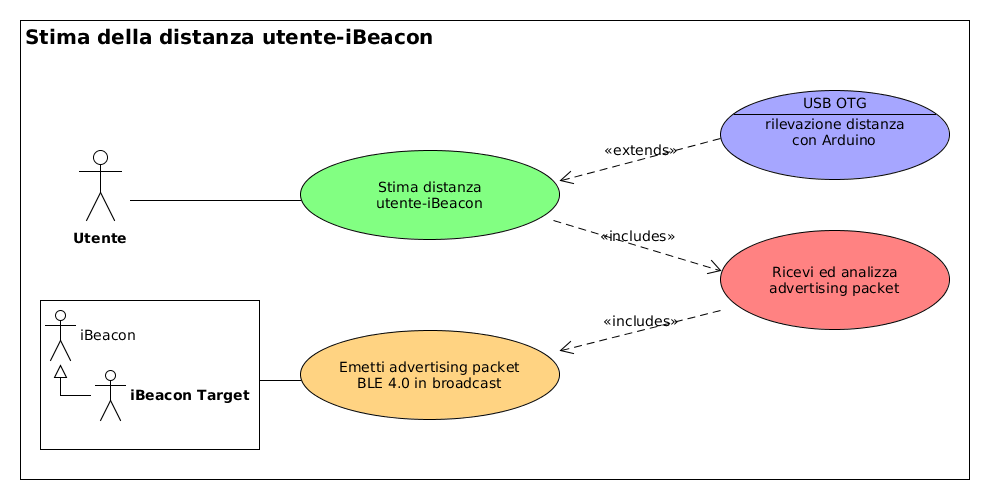
\includegraphics[scale=.45]{img/uml/use_case/use_case1}
	\caption[Use case - Stima della distanza utente-iBeacon]{Use case - Stima della distanza utente-iBeacon}
	\label{fig:usecase}
\end{figure}

\subsection{Scenari}

\subsubsection{\underline{Scenario classico}}
Nello scenario classico l'utente utilizza l'app per scansionare l'ambiente alla ricerca di iBeacon e leggere delle informazioni a schermo.

Nello specifico in questo scenario:
\begin{itemize}
	\item Si considera un utente in una stanza con uno smartphone Android in mano.
	
	\item La stanza in questione può presentare uno o più iBeacon disposti sui muri ad un'altezza di circa 1 metro dal suolo.
	
	\item Sullo smartphone viene avviata l'app.
	
	\item Nel caso in cui la radio Bluetooth dello smarphone fosse spenta o si dovesse spegnere, l'app stessa la accenderà/riaccenderà indicando all'utente l'avvenuto switch.
	
	\item L'utente preme su un bottone per avviare la scansione degli iBeacon presenti.
	
	\item Se vengono rilevati iBeacon corrispondenti con la lista di indirizzi MAC presente nell'app, allora viene caricata una lista di informazioni a schermo (\textit{friendly name}, immagine, distanza stimata, ecc\dots).
\end{itemize}

\subsubsection{\underline{Scenario classico avanzato}}
\begin{itemize}
	\item Una volta che l'utente ha visualizzato l'iBeacon di suo interesse (detto \textit{target}), lo seleziona dalla lista facendo click sull'item corrispondente.
	
	\item A questo punto all'utente vengono proposti solo i dettagli relativi al target, isolandoli dagli altri.
	
	\item In questa sezione l'utente potrebbe visualizzare un feedback della distanza reale (se tutte le condizioni a contorno sono soddisfatte) in metri.
	
	\item Trascinando il dito da destra a sinistra all'utente viene proposta un'altra area ancora più dettagliata dove è possibile mettere a confronto le varie stime della distanza (filtrata, non filtrata e reale se presente) con grafici realizzati in tempo reale.
\end{itemize}

	
	\part{Analisi del problema}
	\chapter{Breve introduzione alla tecnologia iBeacon}
Gli iBeacon (anche detti BLE Beacon) sono dispositivi portatili, spesso alimentati a batteria, che integrano una radio Bluetooth. Il loro scopo è definire \textbf{regioni} di spazio delimitato dall'estensione del segnale che emettono in broadcast ripetutamente con una frequenza predefinita. Si rendono utili per \textit{micro-location system} in quanto offrendo una precisione molto senza forti ripercussioni sulla loro autonomia.

Spesso sono utilizzati come \textit{trigger} per App che integrano \textit{custom action}, reagendo alla prossimità, creando delle reazioni visibili sullo smartphone che utente appaiono come \textbf{interazioni col mondo fisico}.

La tecnologia chiave che permette agli iBeacon di funzionare è la \textbf{proximity specification BLE} (Bluetooth Low Energy), spesso indicata come \textbf{Bluetooth Smart}. BLE è un miglioramento della specifica Bluetooth che permette un consumo energetico ridotto che si ripercuote positivamente sull'autonomia dei dispositivi a batteria.

\begin{figure}[!ht]
	\centering
	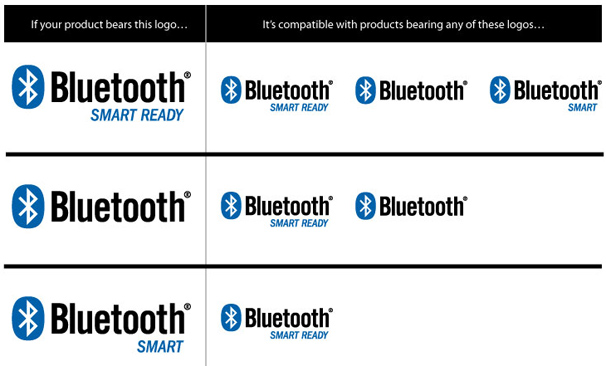
\includegraphics[scale=.25]{img/bt/BT.png}
	\caption{Compatibilità delle diverse tecnologie Bluetooth}
\end{figure}

Il limitato consumo energetico degli iBeacon si deve alla ridotta potenza di trasmissione di questa tecnologia che permette lunghi periodi di utilizzo (mesi o addirittura anni).

\section{Il protocollo iBeacon}
Il protocollo di comunicazione iBeacon è semplice e lineare. Si suddivide tra \textbf{broadcaster} (trasmettitore) e \textbf{receiver} (ricevitore). 

\subsection{Broadcaster}
Nella specifica Bluetooth, un iBeacon è per definizione un \textit{broadcaster}. I broadcaster trasmettono \textbf{advertising packet} periodici che contengono informazioni utilizzabili dai \textit{receiver}. 

\subsection{Receiver}
In questo protocollo i receiver non devono rispondere ai pacchetti che ricevono ed in generale i broadcaster non sono abilitati alla ricezione. La comunicazione degli advertising packet avviene sempre e solo attraverso una trasmissione unidirezionale.

\subsection{Advertising packet}
Essenzialmente gli advertising packet sono dispersi dai broadcaster nell'aria e i receiver possono scegliere se agire o no in base al loro contenuto.

La ricezione di un advertising packet da parte di un receiver provoca la creazione di un \textbf{advertisement event}. Per questo gli advertising packet e gli advertisement event genericamente sono denominati come \textbf{advertisement}. 

\begin{figure}[!ht]
	\centering
	
\includegraphics[scale=.20]{img/bt/ibeacon.png}
	\caption{Logo che identifica i dispositivi iBeacon}
\end{figure}

\section{Frame iBeacon}
Il formato del frame iBeacon è abbastanza semplice. Sono presenti solo un due parametri variabili che sono comunque sufficienti per supportare applicazioni complesse.

Le informazioni che un iBeacon emette si suddividono in tre identificativi:
\begin{itemize}
	\item Universal Unique Identifier
	\item Major number
	\item Minor number
\end{itemize}

\subsection{UUID (128 bits)}
L'UUID identifica univocamente la società di cui l'iBeacon fa parte. A differenza di altri protocolli di rete come 802.11, l'UUID non è gestito centralmente per evitare conflitti. Il protocollo Bluetooth presuppone che UUID siano unici.

L'UUID è il numero più facile da elaborare perché dovrebbe essere unico. Un sistema che supporta più brand name può utilizzare diversi UUID.

La maggior parte degli UUID sono creati da generatori di numeri casuali, spesso integrando l'ora corrente e un identificatore del generatore (ad esempio l'indirizzo MAC). Molte applicazioni per la configurazione di iBeacon commerciali hanno un pulsante per generare un UUID pseudocasuale.

\subsection{Major number (16 bits)}
Le specifiche Bluetooth e iBeacon non dispongono di una struttura per l'uso dei major o minor numers.

Il Major number viene utilizzato per identificare i Major groups di iBeacon di proprietà di un'unica entità. Nell'esempio della catena di negozi, il Major number tipicamente è utilizzato dai iBeacon che si trovano all'interno del negozio, identificando gruppi di proximity area in modo logico. Il campo a 16 bit permette di avere 65.000 possibilità.

\subsection{Minor number (16 bits)}
Il Minor number viene utilizzato per identificare il livello più basso della gerarchia all'interno di un insieme di iBeacon. Tornando all'esempio di una catena di negozi, il Minor number sarà utilizzato per i singoli iBeacon all'interno di una singola posizione del negozio, per esempio potrebbe identificare un prodotto esposto.

Il Minor number è una ulteriore suddivisione del raggruppamento definito dal Major number. I Minor number di solito si riferiscono ad una posizione geografica o POI all'interno di una posizione.

\section{RSSI - Received Signal Strength Indication}
La \textbf{proximity estimation} (stima di prossimità) dipende dal RSSI. RSSI non è trasmesso nel advertising packet, ma viene percepito dal receiver come il livello di potenza del segnale ricevuto.

\subsection{Advertising Interval}
Anche se le specifiche Bluetooth permettono di definire più \textit{advertising interval}, la specifica iBeacon fissa l'advertising interval a 100 ms.

L'impostazione dell'advertising interval è bilanciato in modo da preservare la vita della batteria, ma comunque essere abbastanza lungo per consentire ai servizi basati sugli iBeacon di funzionare.

\section{iBeacon Advertising Packet Contents}
Tutti i advertising packet hanno sempre la stessa lunghezza e sono composti da una serie di campi fissi. L'ultima parte del frame contiene informazioni specifiche del costruttore definito da Apple. È comunque possibile definire un formato pacchetto personalizzato in modo da migliorare le capacità di puntamento un iBeacon.

\begin{figure}[!ht]
	\centering
	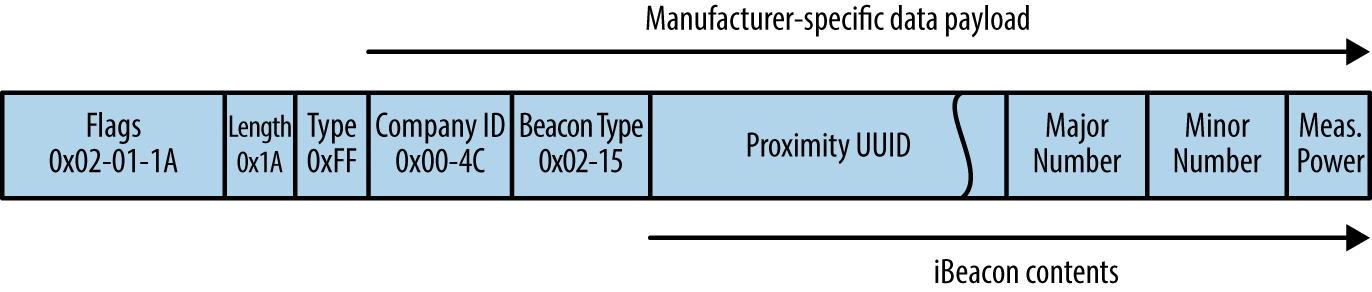
\includegraphics[scale=.25]{img/bt/iBeacon_advertising_packet_format.png}
	\caption{Formato di un iBeacon advertising packet format}
\end{figure}

\subsection{Measured power}
L'idea di \textbf{ranging} è implicita all'interno del protocollo iBeacon. Il \textit{ranging} indica la distanza tra il receiver e l'iBeacon analizzando le variazioni di potenza della trasmissione ricevuta. La distanza da un iBeacon viene stimata in base alla costante di calibrazione adeguata, misurando il tempo che un segnale impiega per poter essere ricevuto e la sua potenza.

Il \textit{Measured power} è un parametro impostato tenendo un receiver ad un metro dall'iBeacon e calcolando la media di RSSI. Questo campo contiene la potenza misurata come complemento a due. 

\paragraph{Esempio:} un valore di C5 indica che la potenza misurata a un metro è di -59 dBm.
\\\\Dati:
\begin{itemize}
	\item \texttt{0xC5\textsubscript{hex} = 197\textsubscript{dec}}
	\item \texttt{0x100\textsubscript{hex} = 256\textsubscript{dec}}
\end{itemize}
\begin{center}
	\texttt{(256 - 197) = -59 dBm}
\end{center}

	\chapter{Stima della distanza con RSSI}

\section{Attenuazione dei segnali elettromagnetici}
Il fenomeno dell'\textbf{attenuazione} dei segnali elettromagnetici si manifesta nella decrescita della potenza di segnale ricevuto dal ricevitore in relazione all’aumentare della distanza dalla sorgente emittente di tale segnale.

Nota questa relazione, se si conosce la potenza di segnale del trasmettitore \textbf{P} è possibile creare un modello per legare l'\textbf{\textit{attenuazione di segnale}} \textbf{A} e la distanza col ricevitore al fine di stimare la \textbf{\textit{distanza relativa}} trasmettitore-ricevitore \textbf{d}.
\begin{equation}\label{eq:realazione_potenza_segnale}
	P = f(d) 
\end{equation}

\section{Received Signal Strength Indicator - RSSI}
Per stimare la distanza relativa tra trasmettitore e ricevitore si può sfruttare l'attenuazione di segnale indicata dal valore RSSI il cui calcolo è poco costoso e non necessita di hardware aggiuntivo. 

RSSI è utile per smartphone che implementano radio Bluetooth in quanto permette di sviluppare proximity app o localizzazione indoor. Il suo valore viene calcolato in automatico dal sistema operativo dello smartphone.

Purtroppo questo approccio non è particolarmente preciso in quanto l’ambiente influisce sulla potenza del segnale ricevuto e quindi sull'attenuazione reale che rende il valore RSSI oscillante.

\begin{figure}[!ht]
	\centering
	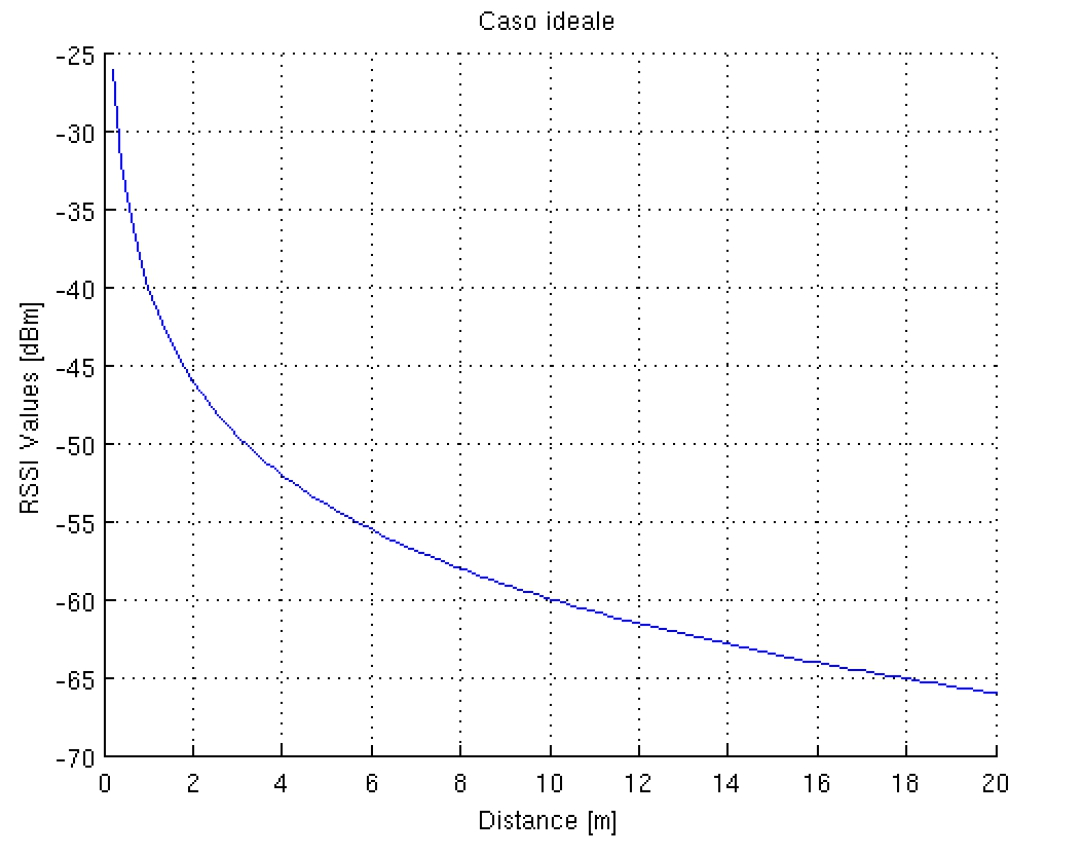
\includegraphics[scale=.25]{img/algoritmi/RSS.png}
	\caption{RSSI - Modello dell'andamento di RSSI in funzione della distanza}
\end{figure}



\section{Calcolo di RSSI}
Per il calcolo di RSSI (in dBm) si assume:
\begin{enumerate}
	\item che un segnale radio emesso in nello spazio libero da ostacoli e rumore decade di un fattore $ d^{-2} $, dove \textbf{d} è la distanza relativa trasmettitore-ricevitore
	
	\item che la potenza media ricevuta attraverso un canale reale decade proporzionalmente a $ n = d^{-n} $ , dove \textbf{n} è detto \textbf{l’esponente path-loss}. Tipicamente \textit{n} è compreso tra 2 e 4.
\end{enumerate}

\subsection{Equazione di trasmissione di Friis}

La distanza dal trasmettitore viene valutata utilizzando l’\textbf{equazione di trasmissione di Friis}:

\begin{equation}\label{eq:potenza_ricevuta}
P_R = P_T \frac{G_T G_R  \lambda^2}{(4 \pi)^2 \textbf{d}^n}
\end{equation}
dove:

\begin{itemize}
	\item $ P_R $ : potenza del segnale ricevuto (espressa in Watt) 
	\item $ P_T $ : potenza del segnale trasmesso (espressa in Watt) 
	\item $ G_R $ : guadagno dell’antenna ricevente
	\item $ G_T $ : guadagno dell’antenna trasmittente
	\item $\lambda = \frac{v}{f}$ : lunghezza d’onda
	\subitem $ v $ : velocità di propagazione
	\subitem $ f $ : frequenza dell'onda 
	\item $ d $ : distanza in metri
	\item $ n $ : constante di propagazione del segnale che dipende dall’ambiente
\end{itemize}
L'equazione \eqref{eq:potenza_ricevuta} calcola il rapporto tra la potenza ricevuta da un'antenna e la potenza trasmessa, in condizioni ideali.

\subsection{Conversione della potenza}
Conversione dalla potenza espressa in watt alla potenza espressa in dBm

\begin{equation}\label{eq:1dBm}
	1_{[dBm]} = 0.001258925_{[W]}
\end{equation}

\begin{equation}\label{eq:1W}
	1_{[W]} = 30_{[dBm]}
\end{equation}

\begin{equation}\label{eq:potenza_in_dBm}
	P_{[dBm]} = 10\log_{10} (10^{3}P_{[W]}/1_{[W]})
\end{equation}

\subsection{Potenza media a distanza di riferimento $ d_0 $}
\begin{equation}\label{eq:potenza_media_a_distanza_d}
	P(d)_{[dBm]} = P_{0\;[dBm]} \left(\frac{d}{d_0} \right)^{-n}
\end{equation}

dove $ P_0 $ è la potenza ricevuta (dBm) a una piccola distanza di riferimento $ d_0 $.

\subsection{Equazione di RSSI}
Combinando la \eqref{eq:potenza_ricevuta} e la \eqref{eq:potenza_in_dBm}, applicando le proprietà dei logaritmi si ottiene:
\begin{equation}
RSSI = −(10\,n\log_{10} \textbf{d} − A)
\end{equation}

dove \textit{A} è la potenza del segnale ricevuto (dBm) a distanza di un metro considerando una costante di propagazione \textit{n}.

\section{Calcolo della distanza}
La seguente equazione permette di stimare la distanza tra l'utente ed un target conoscendo il valore RSSI ed i parametri \textit{A} ed \textit{n}:

\begin{equation}\label{key}
RSSI = P - 10 * n * \log_10(d)
* n = 2 (in free space)
* d = 10 ^ ((TxPower - RSSI) / (10 * n))
\end{equation}

\begin{equation}
\textbf{d} = 10 \left( \frac{A − RSSI}{10\,n} \right)
\end{equation}

Con questa formula si può stimare la distanza .

\section{Problematiche della stima della distanza con RSSI}\label{ch:problematiche}
I principali fenomeni negativi che inficiano l'utilizzo di RSSI come approccio per determinare la distanza tra due punti sono:
\begin{itemize}
	\item \textbf{Riflessione:} il segnale si propaga anche attraverso un percorso riflesso, provocando un \textbf{multi-path fading}. Al ricevitore giungono segnali con ampiezze e fasi differenti che vanno a sommarsi o sottrarsi in funzione della frequenza, causando un fading selettivo. Può essere causato da metalli e altri materiali riflettenti.
	\item \textbf{Intralcio:} shadowing che altera il normale decadimento dell’intensità che si avrebbe in spazio libero. L’attenuazione improvvisa del segnale è causata degli ostacoli (mobili, muri, alberi, edifici, ecc.) nel cammino trasmettitore-ricevitore
	\item \textbf{Assorbimento:} oggetti, come elementi liquidi o corpi umani, che assorbono la potenza del segnale.
	\item \textbf{Altezza:} la differenza di altezza può falsare la stima
	\item \textbf{Orientamento relativo:} il segnale decade se il ricevitore non è direzionato verso l'emettitore
\end{itemize}

\begin{figure}[!ht]
	\centering
	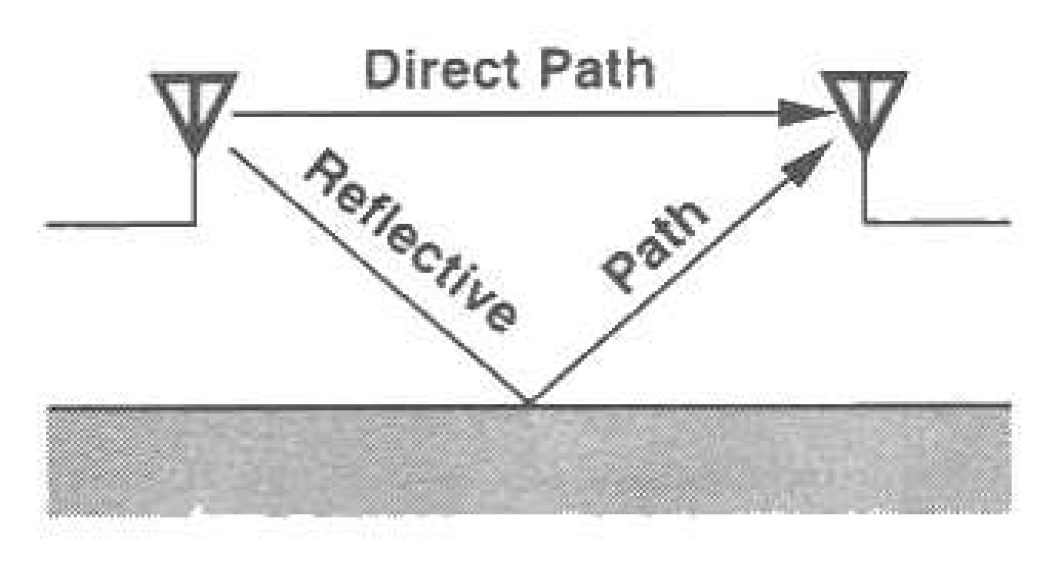
\includegraphics[scale=.16]{img/algoritmi/RSS_PROBLEMI.png}
	\caption{RSSI - Problemi di riflessione}
\end{figure}

\section{Filtro di Kalman}
\begin{quotation}
	\textbf{Definizione 1}: Il filtro di Kalman è stato sviluppato da Rudolf Kalman. 
	La prima realizzazione pratica di questo filtro è stata sviluppata da Stanley Schmidt, che ne riconobbe l'applicabilità per stimare le traiettorie ed eliminare alcuni disturbi.
	
	Teoricamente è uno strumento per stimare lo stato di un sistema dinamico lineare perturbato da rumore sulla base di misure (o osservazioni) che sono linearmente dipendenti dallo stato e corrotte da rumore.
	
	Questo stimatore si definisce \textbf{ottimo} rispetto a qualunque funzione quadratica dell’errore di stima in quanto si basa su tutte le informazioni disponibili.
\end{quotation}
\begin{quotation}
	\textbf{Definizione 2}:	Il filtro di Kalman è una tecnica per la risoluzione del problema Gaussiano lineare quadratico traducibile, indicato come stima dello stato istantaneo di un sistema dinamico a partire dalla sua uscita. Si considera statisticamente ottimale rispetto a qualunque funzione quadratica di stima dell'errore.
	
	Supponendo di conoscere le variabili misurate in funzione delle variabili di interesse, questo filtro si occupa della soluzione del problema inverso, cioè stimando le variabili indipendenti come funzione inversa delle variabili dipendenti (misurabili).
	
	Dato il sistema dinamico:
	
	\begin{equation}
	\begin{cases}
		dX = f ( x(t),u(t),t) \\
		y = h( x(t),u(t),t)
	\end{cases}
	\end{equation}
	Il filtro si occupa di risalire allo stato x(t) a partire dall'uscita y(t) quando queste sono perturbate da rumore gaussiano.
	
	La costruzione del filtraggio dei dati avviene sulla base di una media pesata tra il prossimo valore predetto e il successivo valore stimato.
	
	L'algoritmo e composto da alcune equazioni matematiche che effettuano operazioni ricorsive per dare un efficace soluzione al metodo dei minimi quadrati.
	
	Per la sua costruzione il filtro di Kalman necessita di \textbf{tre ingredienti	fondamentali} vincolati al sistema che si sta studiando:
	\begin{enumerate}
		\item una serie di misure da stimare
		\item un modello matematico descrittivo del sistema
		\item la conoscenza del	modello statistico del sistema
	\end{enumerate}
	
\end{quotation}	

 
 

	\chapter{Stima della distanza con RSSI, Android e tecnologie BLE}

\section{Sviluppare un'app Android compatibile con BLE}
L'obiettivo dell'app è far interagire un cellulare (con sistema operativo Android) con gli iBeacon disposti in una stanza. Dalle API 18 in poi Android integra nativamente la comunicazione e ricezione dati su protocollo Bluetooth LE.

Visto che l'applicazione non funziona senza questa specifica, nell'\texttt{AndroidManifest.xml} sono state imposte delle condizioni che inibiscono l'installazione dell'app a dispositivi che non hanno una radio Bluetooth Low Energy.

\begin{lstlisting}[language=XML]
<uses-permission android:name="android.permission.BLUETOOTH" />
<uses-permission android:name="android.permission.BLUETOOTH_ADMIN" />
<uses-feature android:name="android.hardware.bluetooth_le" android:required="true" />
\end{lstlisting}

Al fine di inibire l'installazione a smartphone con API minori a 18, nel file \texttt{build.gradle} è stata inserita la regola:
\begin{lstlisting}[language=Java]
    defaultConfig {
    	...
    	minSdkVersion 18
    	...
    }
\end{lstlisting}

\section{Compatibilità con Android 5.0+}
Per rendere eseguibile l'app a smarphone con Android dalla versione 5.0 in poi è stato aggiunto un metodo (\texttt{checkAndroidMPermission()}) per fare il check dei permessi di Android. Senza questo accorgimento l'app sarebbe stata installata ma non avrebbe funzionato la scansione dei dispositivi BT.

\subsubsection{Controllo della compatibilità con Android 5.0+}
\begin{lstlisting}[language=Java]
private void checkAndroidMPermission() {
   	
   	if (Build.VERSION.SDK_INT >= Build.VERSION_CODES.M) {
   		final List<String> permissions = new ArrayList<>();
   		
   		if (checkSelfPermission(Manifest.permission
		   	.ACCESS_FINE_LOCATION)
		   		!= PackageManager.PERMISSION_GRANTED) {
   			permissions.add(Manifest.permission
	   			.ACCESS_FINE_LOCATION);
   		}
   		
   		if (checkSelfPermission(Manifest.permission
	   		.ACCESS_COARSE_LOCATION)
		   		!= PackageManager.PERMISSION_GRANTED) {
   			permissions.add(Manifest.permission
	   			.ACCESS_COARSE_LOCATION);
   		}
   		
   		if (!permissions.isEmpty()) {
   			new AlertDialog.Builder(this)
   			.setTitle(R.string.dialog_location_access_title)
   			.setMessage(R.string.dialog_bluetooth_text)
   			.setPositiveButton(android.R.string.ok, null)
   			.setOnDismissListener(new DialogInterface.OnDismissListener() {
   				@TargetApi(23)
   				@Override
   				public void onDismiss(DialogInterface dialog) {
   					requestPermissions(permissions.toArray(
	   					new String[permissions.size()]),
   					REQUEST_CODE_ASK_MULTIPLE_PERMISSIONS);
   				}
   				
   			}).show();
   		}
   	}
}
\end{lstlisting}

\section{Libreria AltBeacon - android-beacon-library}
Per estendere il supporto nativo fornito alla connettività Bluetooth è stata utilizzata la libreria \href{https://github.com/AltBeacon/android-beacon-library}{\textbf{AltBeacon}}\footnote{\href{https://github.com/AltBeacon/android-beacon-library}{\textbf{AltBeacon}} - \url{https://github.com/AltBeacon/android-beacon-library}}. Questa permette di generare delle regioni di interesse, degli avvisi all'utente, filtrare i dispositivi BT, ecc. Con essa è inoltre fornito un modulo per il risparmio energetico.

Per l'inclusione di questa libreria si inserita la seguente stringa nel file \texttt{build.gradle}.
\begin{lstlisting}[language=Java]
dependencies {
	...
	// android beacon library AltBeacon
	compile 'org.altbeacon:android-beacon-library:2.9.1'
	...
}
\end{lstlisting}

\section{Calcolo della distanza RAW}
La stima della distanza in base ai RSSI calcolati si esegue nel metodo \texttt{calculateDistance(double txPower, double rssi)}.

\subsubsection{Stima della distanza in base agli RSSI}
\begin{lstlisting}[language=Java]
// radiousNetwork formula
private double calculateDistance(double txPower, double rssi) {
	
	if (rssi == 0.0D) {
		return -1.0D; // if we cannot determine accuracy, return -1.
	}
	
	double ratio = (rssi * 1.0D) / txPower;
	if (ratio < 1.0D) {
		return Math.pow(ratio, 10.0D);
	}
	
	return (0.89976D * Math.pow(ratio, 7.7095D)) + 0.111D;
}
\end{lstlisting}

\section{Filtri}
Per ridurre le problematiche di rilevamento di RSSI(\ref{ch:problematiche}) sono stati sviluppati e/o utilizzati tre filtri: RunningAverageRssi, filtro di Kalman, filtro ARMA. Questi possono essere combinati tra loro senza inficiare le prestazioni del sistema. Presentano delle parametrizzazioni controllabili dal \textit{Settings} per adattarsi a tutti vari contesti di stima.

Per scelta progettuale il filtro di Kalman è sempre attivo. Si è fatto in modo che il valore filtrato col questo filtro sia confrontabile con la misurazione della distanza RAW e con quella filtrata dalla libreria AltBeacon.

\subsection{Filtro RunningAverageRssi}
Il filtro \textit{RunningAverageRssi} calcola il valore RSSI sulla base di un elenco arbitrario di valori RSSI misurati. L'elenco viene troncato da una certa lunghezza all'inizio e alla fine. Il valore calcolato è una semplice media aritmetica. Viene fornito dalla libreria AltBeacon come filtro di default, ma non sembra essere particolarmente preciso.

\subsection{Implementazione del filtro di Kalman}

Per realizzare il filtro di Kalman sono state utilizzate tre classi: 
\begin{itemize}
	\item \texttt{KFilterBuilder}: per creare un filtro di Kalman unidimensionale;
	\item \texttt{KFilter}: per il filtraggio vero e proprio.
	\item \texttt{Estimation}: per implementare il filtro sui valori di input.
\end{itemize}
Parametri passati a KFilter:
\begin{itemize}
	\item R = rumore di processo;
	\item Q = misurazione del rumore;
	\item A = vettore di stato;
	\item B = vettore di controllo;
	\item C = vettore delle misurazioni.
\end{itemize}

Questo filtro è inizializzato nella classe \texttt{Estimation} (istanziata volta alla creazione di degli oggetti \textit{Device}). Ogni volta che viene richiamato il metodo \texttt{updateDistance(Beacon b, double processNoise)} di \texttt{EStimation};
\begin{itemize}
	\item si aggiunge un nuovo valore alla variabile \texttt{recentRSSI}, istanza di un oggetto \texttt{DescriptiveStatistics}
	\item si aggiunge un nuovo valore alla variabile \texttt{recentTxPower}, istanza di un oggetto \texttt{DescriptiveStatistics}
	\item si calcola il nuovo valore di rumore in base ai nuovi input
	\item se il nuovo valore di rumore non è un numero infinito e non è un Not-a-Number, si passa al metodo \texttt{setMeasurementNoise(mNoise)} di \texttt{KFilter}
	\item si setta il nuovo rumore di processo, che dipende dall'input dato da \texttt{Settings}
	\item si calcola la distanza con i parametri appena calcolati
\end{itemize}

\subsubsection{Filtraggio in base agli input}
\begin{lstlisting}[language=Java]
public void updateDistance(Beacon b, double processNoise) {
   	
   	recentRSSI.addValue(b.getRssi());
   	recentTxPower.addValue(b.getTxPower());
   	
   	// Update measurement noise continually
   	double mNoise = Math.sqrt((100 * 9 / Math.log(10)) *
   	Math.log(1 + Math.pow(recentRSSI.getMean() / recentRSSI.getStandardDeviation(), 2)));
   	
   	if (!Double.isInfinite(mNoise) && !Double.isNaN(mNoise)) {
   		kf.setMeasurementNoise(mNoise);
   	}
   	
   	kf.setProcessNoise(processNoise);
   	double lastFilteredReading = kf.filter(recentRSSI.getPercentile(50));
   	distanceEstimated = calculateDistance(recentTxPower.getPercentile(50), lastFilteredReading);
   	rawDistanceEstimated = calculateDistance(b.getTxPower(), b.getRssi());
   	WOSC = calculateDistance(b.getTxPower(), lastFilteredReading);
}
\end{lstlisting}

\subsubsection{Filtering nella classe KFilter}\label{ch:kfilter}
\begin{lstlisting}[language=Java]
/**
* Filter a new value
*
* @param z Measurement
* @param u Control
* @return x
*/
public double filter(double z, double u) {
   	
   	if (Double.isNaN(x)) {
   		x = (1 / C) * z;
   		x1 = x;
   		x2 = x1;
   		cov = (1 / C) * Q * (1 / C);
   	} else {
   	
    	// Calculate previous update step
    	B = (x - x1) / 2;
   	
    	// Compute prediction
    	double predX = (A * x) + (B * u);
    	double predCov = ((A * cov) * A) + R;
   	
    	// Kalman gain
    	double K = predCov * C * (1 / ((C * predCov * C) + Q));
    	
    	// Correction
    	x1 = x;
    	x = predX + K * (z - (C * predX));
    	cov = predCov - (K * C * predCov);
	}

	return x;
}
\end{lstlisting}

\subsection{Implementazione del filtro ARMA}\label{ch:filtro_arma}
Il filtro \textbf{ARMA} (\textit{Auto Regressive Moving Average}) calcola gli RSSI in base al valore corrente. Questo filtro è tradotto in codice nella classe \texttt{MyArmaRssiFilter} che implementa la classe \texttt{RssiFilter}.

Per il filtraggio degli RSSI si utilizza la formula\ref{eq:arma}:
\begin{equation}\label {eq:arma}
n(t) = n(t-1) - c (n(t-1) - n(t))
\end{equation} 
dove $ c $ è il coefficiente che denota l'uniformità (\textit{smoothness}). Più basso è questo valore più uniforme è la media.

Il metodo più importante di questa classe è \texttt{addMeasurement(Integer rssi)} dove si ricevono in input gli RSSI e si esegue il filtraggio in base al coefficiente $ c $ (qui tradotto nella variabile \texttt{armaSpeed}).

\subsubsection{Aggiornamento del filtro ARMA}
\begin{lstlisting}[language=Java]
@Override
public void addMeasurement(Integer rssi) {
    	
   	if (isEnabled) {
   		if (!isInitialized) {
   			armaMeasurement = rssi;
   			isInitialized = true;
   		}
   		armaMeasurement = (armaMeasurement - armaSpeed * (armaMeasurement - rssi));
   	} else {
    	armaMeasurement = rssi;
    }
}
\end{lstlisting}

Per il settaggio dinamico del coefficiente $ c $ si utilizza il metodo \texttt{setArmaSpeed(double arma\_speed)}. Visto che i segnali considerati tendono a variare piuttosto frequentemente (alla frequenza di 1Hz o superiore), il valore consigliato per 1HZ sarebbe 0,1 (cioè l'input viene modificato del 10\% della differenza tra la misurazione attuale e la media effettiva). Per segnali a frequenza superiori (10Hz) si consiglia un valore compreso tra 0,25 e 0,5.

\subsection{Grafici in tempo reale}
Si è scelto di far visualizzare a schermo, direttamente dall'app, dei grafici in tempo reale in modo da rendere più chiaro l'andamento delle stime.
Per far questo è stata utilizzata la libreria \href{https://github.com/PhilJay/MPAndroidChart}{\textbf{MPAndroidChart}}\footnote{\href{https://github.com/PhilJay/MPAndroidChart}{\textbf{MPAndroidChart}} - \url{https://github.com/PhilJay/MPAndroidChart}}.

Per l'inclusione di questa libreria si inserita la seguente stringa nel file \texttt{build.gradle}.
\begin{lstlisting}[language=Java]
dependencies {
	...
	// chart library
	compile 'com.github.PhilJay:MPAndroidChart:v3.0.0-beta1'
	...
}
\end{lstlisting}

\subsubsection{Dettaglio di un grafico in tempo reale}
\begin{figure}[ph]
	\centering
	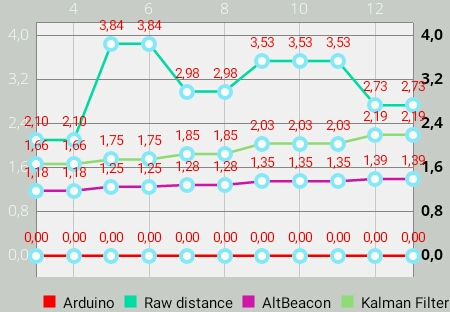
\includegraphics[width=0.6\linewidth]{img/app/chart1.jpg}
	\caption{Esempio di grafico in tempo reale}
	\label{fig:chart1}
\end{figure}




	\chapter{Stima della distanza con Arduino}
\section{Progetto per stimare la distanza con un sensore ultrasonico ed un Arduino}
Per poter stimare la distanza con Arduino è stato utilizzato un sensore ultrasonico. Questo sensore è stato connesso direttamente alla board attraverso cavi maschio-femmina.

\begin{lstlisting}[language=XML]
<intent-filter>
	<action android:name="android.intent.action.MAIN" />
	<action android:name="android.hardware.usb.action
		.USB_DEVICE_ATTACHED"/>

	<category android:name="android.intent.category.DEFAULT" />
	<category android:name="android.intent.category.LAUNCHER" />

</intent-filter>

<meta-data android:name="android.hardware.usb.action
		.USB_DEVICE_ATTACHED" 
	android:resource="@xml/device_filter" />
\end{lstlisting}



\begin{itemize}
	 \item Implementare un progetto Arduino che faccia uso della libreria \href{http://playground.arduino.cc/Code/NewPing}{\textbf{NewPing}}\footnote{\href{http://playground.arduino.cc/Code/NewPing}{\textbf{NewPing}} - \url{http://playground.arduino.cc/Code/NewPing}};
	 
	 \item Sfruttare la libreria \href{https://github.com/mik3y/usb-serial-for-android}{\textbf{usb-serial-for-android}}\footnote{\href{https://github.com/mik3y/usb-serial-for-android}{\textbf{usb-serial-for-android}} - \url{https://github.com/mik3y/usb-serial-for-android}} per connettere l'Arduino ad Android e ricevere i dati seriali in tempo reale.
	 
	 \item Sviluppare un mini progetto su \href{https://netbeans.org/}{\textbf{NetBeans}}\footnote{\href{https://netbeans.org/}{\textbf{NetBeans}} - \url{https://netbeans.org/}} ed impiegare la libreria \href{https://github.com/scream3r/java-simple-serial-connector}{\textbf{jSSC}}\footnote{\href{https://github.com/scream3r/java-simple-serial-connector}{\textbf{jSSC}} - \url{https://github.com/scream3r/java-simple-serial-connector}} (\textit{java-simple-serial-connector}) per testare il sensore di prossimità collegando l'Arduino al PC e visualizzando la distanza a schermo.
\end{itemize}

\subsubsection{\underline{\href{http://playground.arduino.cc/Code/NewPing}{NewPing}}}\label{sec:newping}
\textbf{Caratteristiche}
\begin{itemize}
	\item Compatibile con diversi modelli di sensori ad ultrasuoni: SR04, SRF05, SRF06, DYP-ME007 e Parallax Ping™.
	
	\item Non soffre di \textbf{lag} di un secondo se non si riceve un ping di eco.
	
	\item Produce un ping coerente e affidabile fino a 30 volte al secondo.
	
	\item Timer interrupt method per sketch event-driven.
	
	\item Metodo di filtro digitale built-in \texttt{ping\_median()} per facilitare la correzione degli errori.
	
	\item Utilizzo dei registri delle porte durante l'accesso ai pin per avere un'esecuzione più veloce e dimensioni del codice ridotte.
	
	\item Consente l'impostazione di una massima distanza di lettura del ping "in chiaro".
	
	\item Facilita l'utilizzo di più sensori.
	
	\item Calcolo distanza preciso, in centimetri, pollici e uS.
	
	\item Non fa uso di \texttt{pulseIn}, metodo che risulterebbe lento e che con alcuni modelli di sensore a ultrasuoni restituisce risultati errati.
	
	\item Attualmente in sviluppo, con caratteristiche che vengono aggiunte e bug/issues affrontati.
\end{itemize}

\section{Progetto di test della comunicazione seriale PC - Arduino}
Il metodo più importante di questo mini progetto è \texttt{updateDistance()}. Questo metodo è di tipo \textbf{void}. Il suo scopo è quello di riceve in input i \textit{byte} dalla porta seriale e convertirli in stringhe da visualizzare a schermo su una \textit{jLabel}.

Per poter fare I/O sulla porta seriale si deve istanziare e configurare l'oggetto SerialPort, abilitando la comunicazione via USB con una board Arduino.

Per avviare la comunicazione:
\begin{itemize}
	\item si settano i parametri di ingaggio (baund rate, numero di bit dei pacchetti, numero dei bit di stop e se è presente un controllo di parità)
	
	\item si imposta l'event mask in modo da controllare se sul canale sono prenti \textit{char}
	
	\item si registra l'istanza di SerialPort in un listener di eventi di I/O della seriale per poi considerare solo i dati di tipo \textit{char} e scartare tutti gli altri. 
\end{itemize}


Metodo updateDistance()
\begin{lstlisting}[language=Java]
private void updateDistance() {    
	SerialPort serialPort = new SerialPort("/dev/ttyACM0");
	try {
		serialPort.openPort();
		
		serialPort.setParams( 
			SerialPort.BAUDRATE_115200, 
			SerialPort.DATABITS_8, 
			SerialPort.STOPBITS_1,
			SerialPort.PARITY_NONE);
			
		serialPort.setEventsMask(SerialPort.MASK_RXCHAR);
		
		serialPort.addEventListener((SerialPortEvent serialPortEvent) -> {
			if (serialPortEvent.isRXCHAR()) {
				try {
					Thread.sleep(20);
					String distance = serialPort.readString();
					jLabel1.setText(distance);
				} catch (SerialPortException | InterruptedException ex) {
				}
			}
		});
	} catch (SerialPortException ex) {
		System.out.println("SerialPortException: " + ex.toString());
	}
}
\end{lstlisting}


	
	\part{Progetto}
	\chapter{Gerarchia delle classi}

\section{MainActivity}
\begin{figure}[ph]
	\centering
	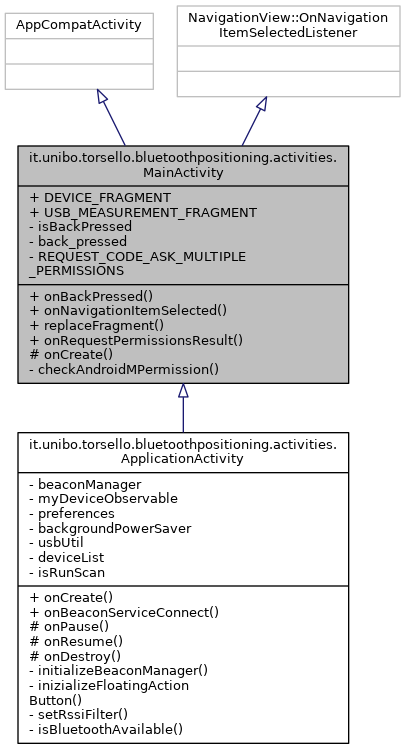
\includegraphics[width=0.40\linewidth]{img/uml/class/classit_1_1unibo_1_1torsello_1_1bluetoothpositioning_1_1activities_1_1MainActivity__inherit__graph.png}
	\caption{Classe - MainActivity}
\end{figure}
La classe \texttt{Main} viene istanziata per prima all'avvio dell'app. Serve ad inizializzare gli oggetti grafici, controllare la compatibilità con Android 5.0+ e rimpiazzare i fragment da visualizzare selezionati dal menu a sinistra.

\begin{figure}[ph]
	\centering
	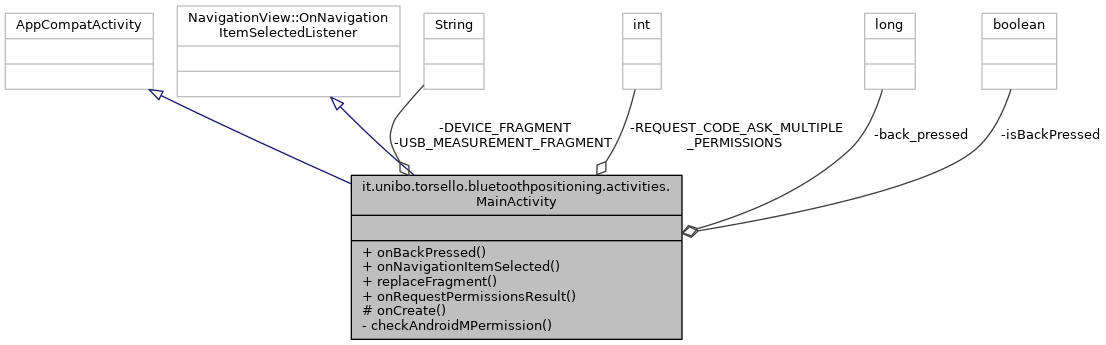
\includegraphics[width=1.8\linewidth,angle=90]{img/uml/class/classit_1_1unibo_1_1torsello_1_1bluetoothpositioning_1_1activities_1_1MainActivity__coll__graph.png}
	\caption{Collaborazione - MainActivity}
\end{figure}

\newpage
\section{ApplicationActivity}
\begin{figure}[ph]
	\centering
	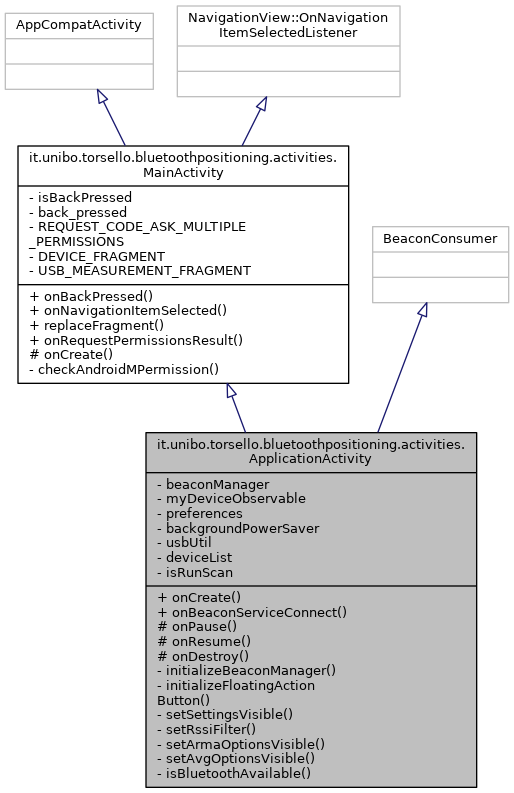
\includegraphics[width=0.7\linewidth]{img/uml/class/classit_1_1unibo_1_1torsello_1_1bluetoothpositioning_1_1activities_1_1ApplicationActivity__inherit__graph.png}
	\caption{Classe - ApplicationActivity}
\end{figure}

Questa classe è una parte fondamentale del progetto. Qui si istanzia e controlla l'oggetto \texttt{BeaconManager} responsabile dello scanning su BT e quindi si ricevono le informazioni dei dispositivi vicini.

Alla ricezione dei dati, questi vengono spediti al \texttt{DeviceObservable} a cui tutti gli Observer interessati si registreranno in modo da ottenere tutti lo stesso valore aggiornato.

\begin{figure}[ph]
	\centering
	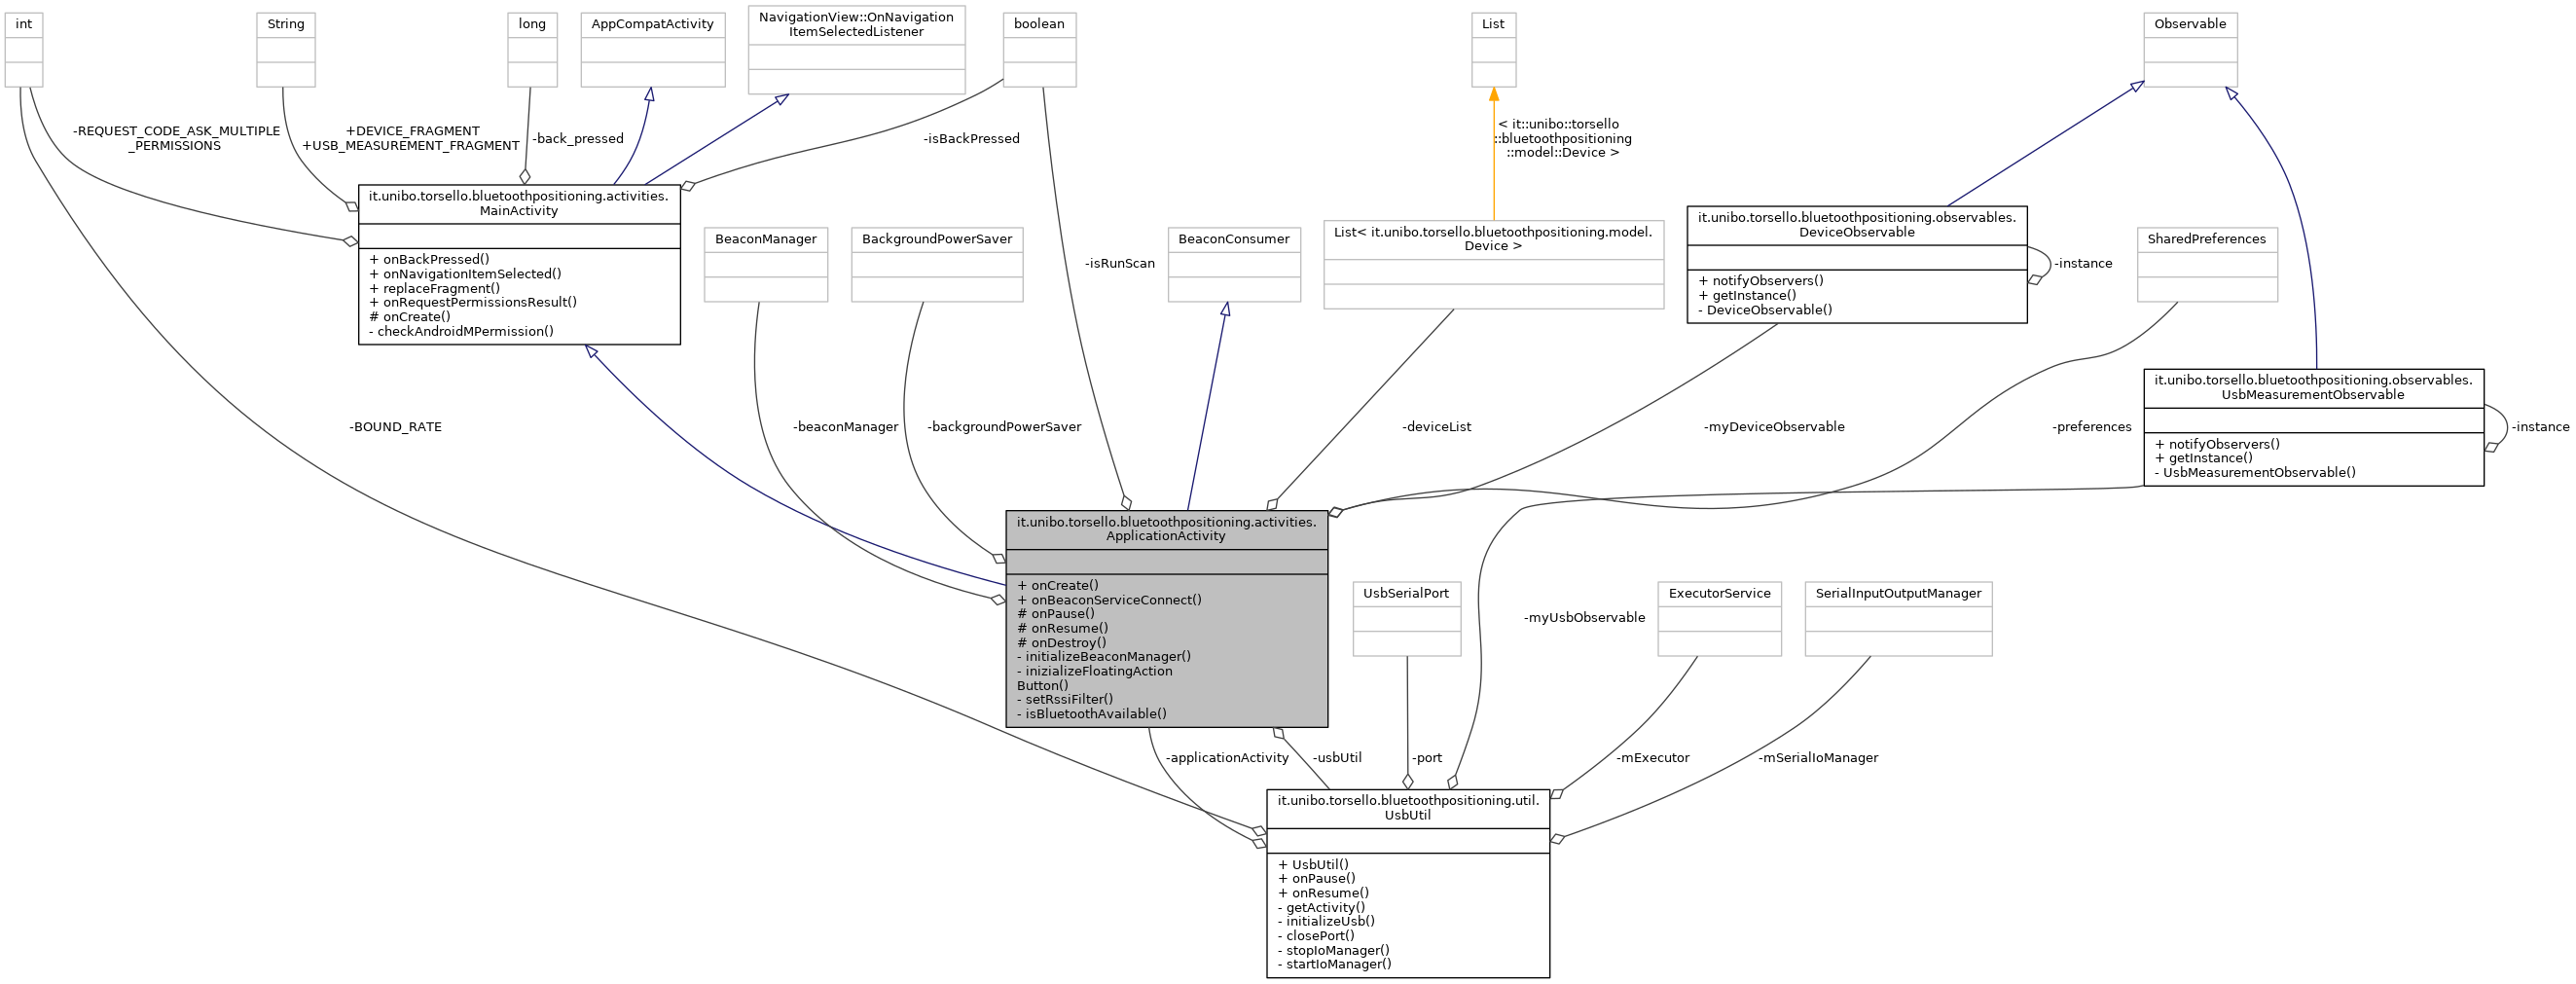
\includegraphics[width=1.9\linewidth, angle=90]{img/uml/class/classit_1_1unibo_1_1torsello_1_1bluetoothpositioning_1_1activities_1_1ApplicationActivity__coll__graph.png}
	\caption{Collaborazione - ApplicationActivity}
\end{figure}

\newpage
\section{Device}
\begin{figure}[ph]
	\centering
	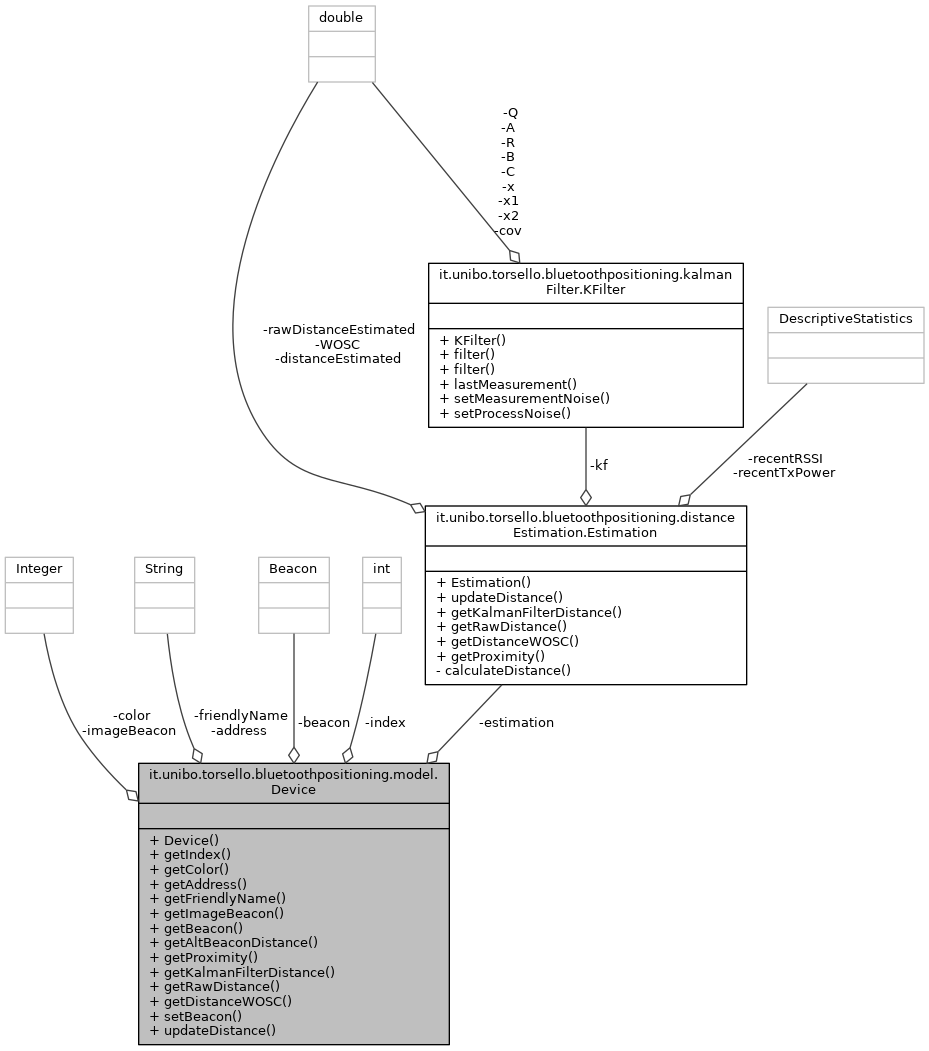
\includegraphics[width=0.9\linewidth]{img/uml/class/classit_1_1unibo_1_1torsello_1_1bluetoothpositioning_1_1model_1_1Device__coll__graph.png}
	\caption{Collaborazione - Device}
\end{figure}

Classe che modella la definizione di dispositivo Bluetooth BLE nel sistema. Alcuni dei dati presenti nella classe sono inizializzati alla creazione che avviene nella classe \texttt{DeviceConstants}, altri sono invece calcolati durante l'esecuzione, come la stima della distanza da parte dei vari filtri.

\newpage
\section{DeviceConstants}
\begin{figure}[ph]
	\centering
	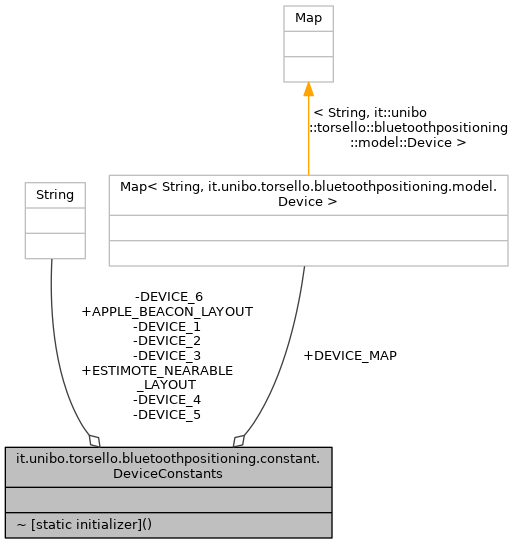
\includegraphics[width=0.7\linewidth]{img/uml/class/classit_1_1unibo_1_1torsello_1_1bluetoothpositioning_1_1constant_1_1DeviceConstants__coll__graph.png}
	\caption{Collaborazione - DeviceConstants}
\end{figure}

Classe che modella ed inizializza i dispositivi sotto forma di oggetto \texttt{Device}. Al suo interno è presente una \texttt{Map} in cui sono indicati i soli ed unici dispositivi che saranno riconosciuti dal sistema.

\newpage
\section{DeviceObservable}
\begin{figure}[ph]
	\centering
	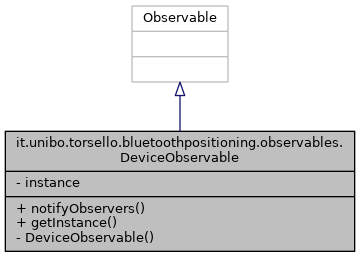
\includegraphics[width=0.7\linewidth]{img/uml/class/classit_1_1unibo_1_1torsello_1_1bluetoothpositioning_1_1observables_1_1DeviceObservable__inherit__graph.png}
	\caption{Classe - DeviceObservable}
\end{figure}

Lo scopo di questa classe è creare un Observable che notifichi a tutti gli Observer registrati l'oggetto list con tutti gli update dei dispositivi scansionati. Questa lista viene aggiornata nella classe \texttt{ApplicationActivity} nel metodo \texttt{onBeaconServiceConnect}

\newpage
\section{Estimation}
\begin{figure}[ph]
	\centering
	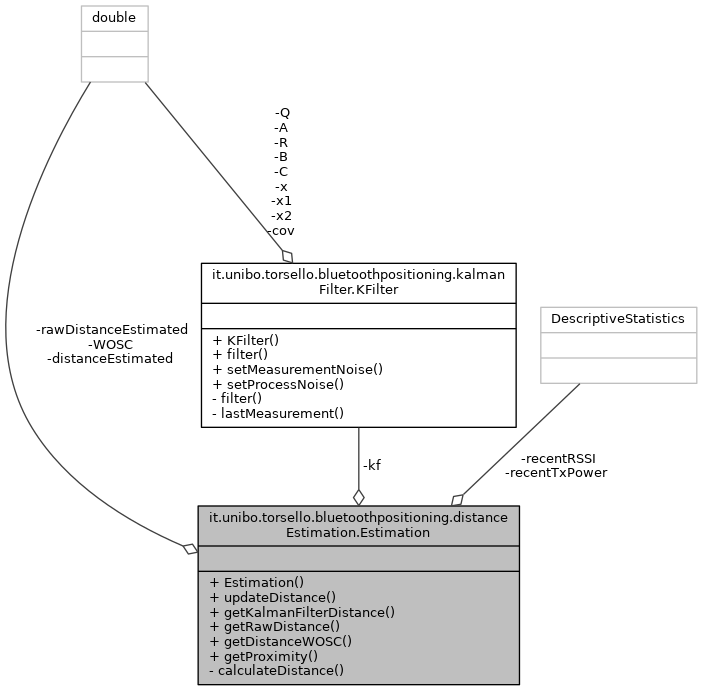
\includegraphics[width=1.2\linewidth]{img/uml/class/classit_1_1unibo_1_1torsello_1_1bluetoothpositioning_1_1distanceEstimation_1_1Estimation__coll__graph.png}
	\caption{Collaborazione - Estimation}
\end{figure}

\newpage
\section{SettingsFragment}
\begin{figure}[ph]
	\centering
	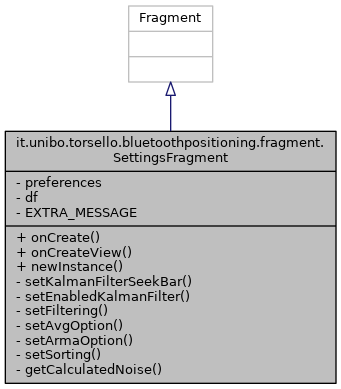
\includegraphics[width=0.5\linewidth]{img/uml/class/classit_1_1unibo_1_1torsello_1_1bluetoothpositioning_1_1fragment_1_1SettingsFragment__inherit__graph.png}
	\caption{Classe - SettingsFragment}
\end{figure}

Classe che implementa Fragment per creare una vista disposta in un menu a destra. Il suo scopo è permettere all'utente di interagire con l'app e con il sistema fisico in cui ci si esegue la stima modificando dei semplici parametri.

\newpage
Nel particolare si usa l'oggetto \texttt{SharedPreferences} per salvare le impostazioni utilizzate. Nel caso in cui l'app fosse chiusa, le impostazioni salvate precedentemente vengono reimpostate come se l'app non fosse mai stata terminata.

\begin{figure}[ph]
	\centering
	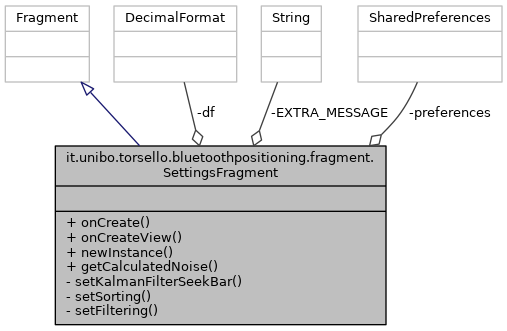
\includegraphics[width=0.8\linewidth]{img/uml/class/classit_1_1unibo_1_1torsello_1_1bluetoothpositioning_1_1fragment_1_1SettingsFragment__coll__graph.png}
	\caption{Collaborazione - SettingsFragment}
\end{figure}

\newpage
\section{SettingConstants}

Classe in cui si settano le costanti relative ai settaggi. Tali costanti sono intese come chiavi per risalire alle impostazioni scelte dall'utente, come ad esempio il filtro o l'ordinamento dei dispositivi trovati.
\begin{figure}[ph]
	\centering
	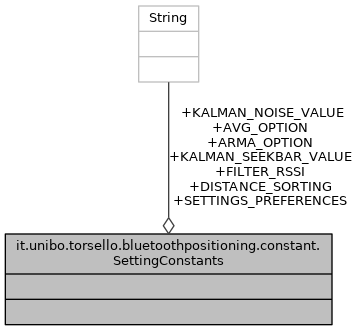
\includegraphics[width=0.5\linewidth]{img/uml/class/classit_1_1unibo_1_1torsello_1_1bluetoothpositioning_1_1constant_1_1SettingConstants__coll__graph.png}
	\caption{Collaborazione - SettingConstants}
\end{figure}

\newpage
\section{DeviceListFragment}\label{ch:device_list}
\begin{figure}[ph]
	\centering
	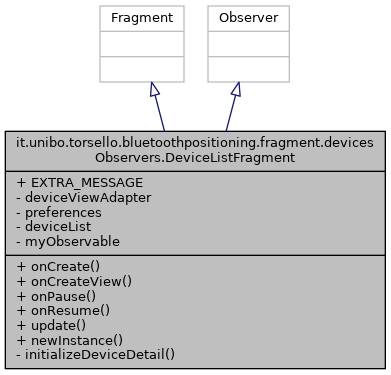
\includegraphics[width=0.5\linewidth]{img/uml/class/classit_1_1unibo_1_1torsello_1_1bluetoothpositioning_1_1fragment_1_1devicesObservers_1_1DeviceListFragment__inherit__graph.png}
	\caption{Classe - DeviceListFragment}
\end{figure}

Classe che aggiorna la lista dei dispositivi con le nuove informazioni ricevute dal metodo \texttt{update(...)}, \textit{override} della classe Observer.
\begin{lstlisting}[language=Java]
@Override
publilc void update(Observable o, Object arg) {
	
	if (arg instanceof List) {
		
		if (!deviceList.isEmpty()) {
			deviceList.clear();
		}
		
		List<Device> devices = (List<Device>) arg;
		
		// optional sorting
		Collections.sort(devices, new Comparator<Device>() {
			public int compare(Device b1, Device b2) {
				int sorting = preferences
					.getInt(SettingConstants.DISTANCE_SORTING, 0);
				switch (sorting) {
					case 0:
					case R.id.radioButton_default_sorting:
					return Double.compare(b1.getIndex(), b2.getIndex());
					case R.id.radioButton_color_sorting:
					return Double.compare(b1.getColor(), b2.getColor());
					case R.id.radioButton_distance_sorting:
					return Double.compare(b1.getKalmanFilterDistance(), b2.getKalmanFilterDistance());
				} // default sorting (a good basic ordering for the other options)
				return Double.compare(b1.getIndex(), 
						b2.getIndex());
			}
		});
		
		deviceList.addAll(devices);
		deviceViewAdapter.notifyDataSetChanged();
	}
}
\end{lstlisting}

Nel dettaglio si aggiorna la lista in base alle preferenze impostate in \texttt{Settings}.

\begin{figure}[ph]
	\centering
	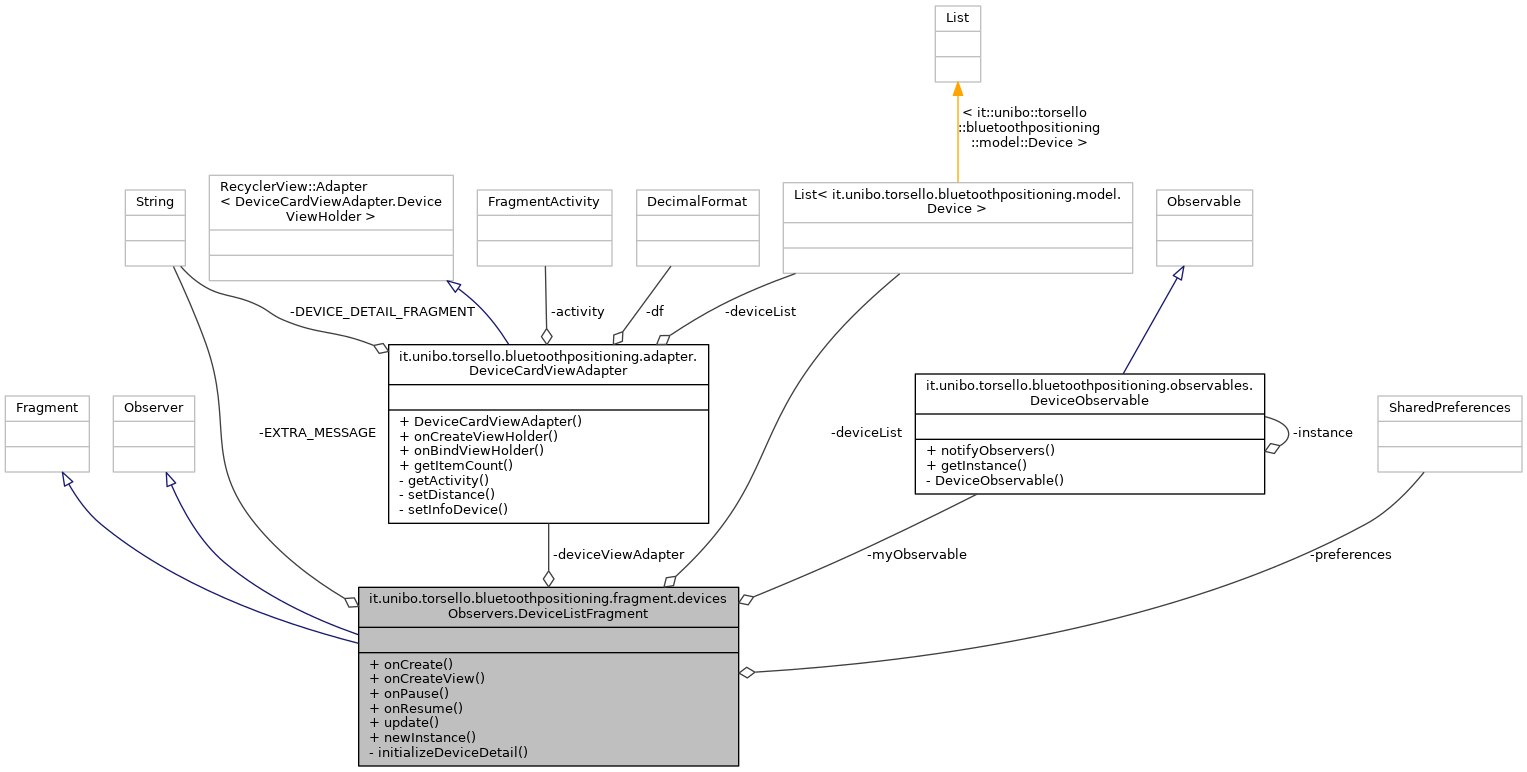
\includegraphics[width=1.9\linewidth,angle=90]{img/uml/class/classit_1_1unibo_1_1torsello_1_1bluetoothpositioning_1_1fragment_1_1devicesObservers_1_1DeviceListFragment__coll__graph.png}
	\caption{Collaborazione - DeviceListFragment}
\end{figure}

\newpage
\section{DeviceCardViewAdapter}
\begin{figure}[ph]
	\centering
	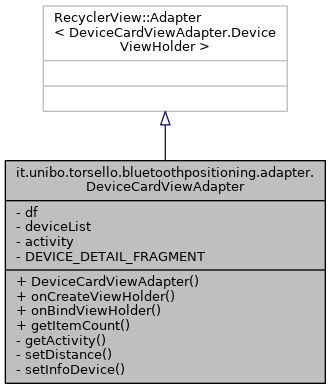
\includegraphics[width=0.5\linewidth]{img/uml/class/classit_1_1unibo_1_1torsello_1_1bluetoothpositioning_1_1adapter_1_1DeviceCardViewAdapter__inherit__graph.png}
	\caption{Classe - DeviceCardViewAdapter}
\end{figure}

Classe responsabile della visualizzazione delle nuove informazioni a schermo. Qui si gestiscono gli elementi grafici da fare vedere o nascondere (valori testuali o immagini) nella RecyclerView.

Viene utilizzata nella schermata principale e nel fragment dei dettagli.

\begin{figure}[ph]
	\centering
	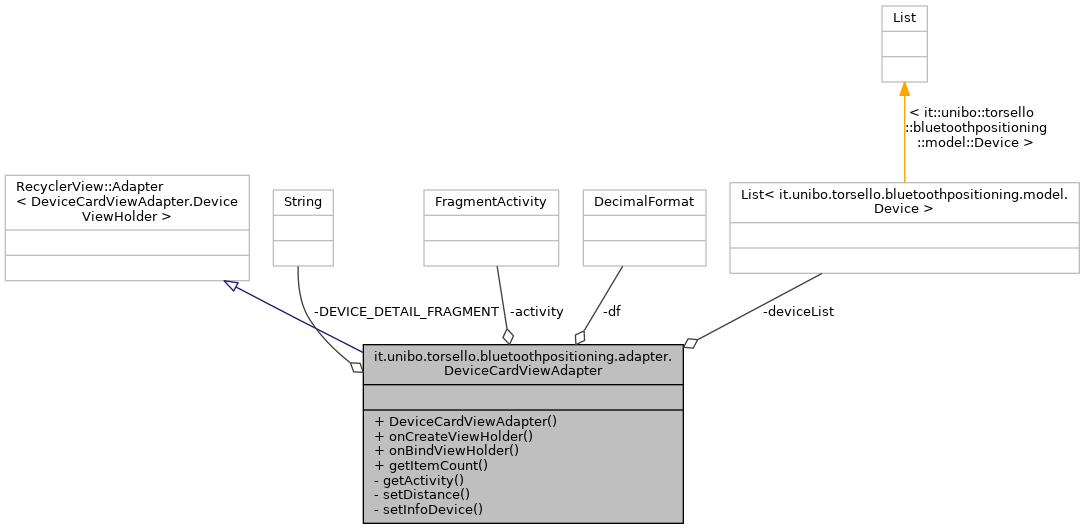
\includegraphics[width=1.5\linewidth,angle=90]{img/uml/class/classit_1_1unibo_1_1torsello_1_1bluetoothpositioning_1_1adapter_1_1DeviceCardViewAdapter__coll__graph.png}
	\caption{Collaborazione - DeviceCardViewAdapter}
\end{figure}

\newpage
\section{DeviceViewHolder}
\begin{figure}[ph]
	\centering
	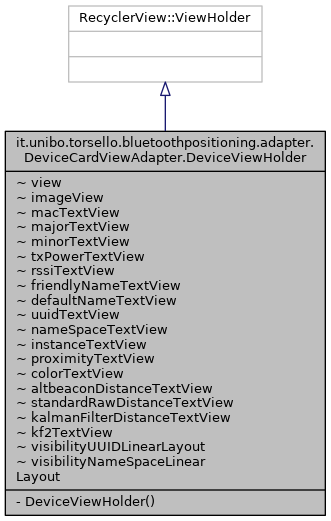
\includegraphics[width=0.5\linewidth]{img/uml/class/classit_1_1unibo_1_1torsello_1_1bluetoothpositioning_1_1adapter_1_1DeviceCardViewAdapter_1_1DeviceViewHolder__inherit__graph.png}
	\caption{Classe - DeviceViewHolder}
\end{figure}

Classe che serve ad inizializzare i vari oggetti grafici da visualizzare nel RecyclerView, risparmiando memoria.

\begin{figure}[ph]
	\centering
	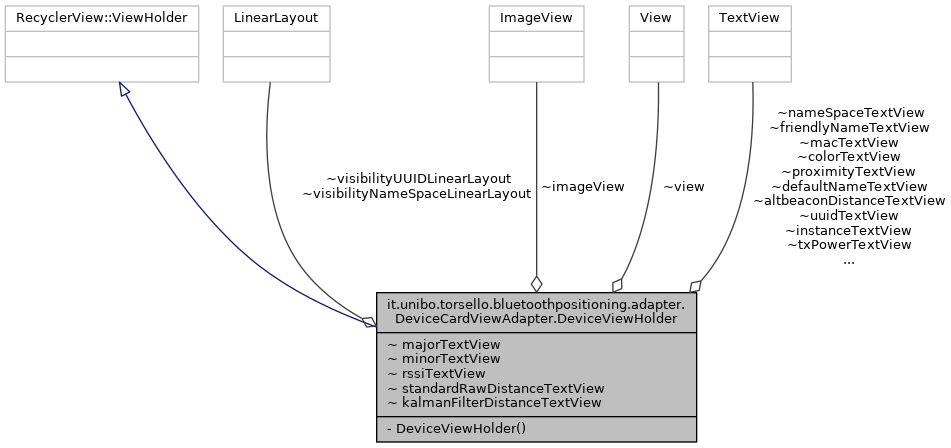
\includegraphics[width=1.5\linewidth,angle=90]{img/uml/class/classit_1_1unibo_1_1torsello_1_1bluetoothpositioning_1_1adapter_1_1DeviceCardViewAdapter_1_1DeviceViewHolder__coll__graph.png}
	\caption{Collaborazione - DeviceViewHolder}
\end{figure}

\newpage
\section{MyArmaRssiFilter}
\begin{figure}[ph]
	\centering
	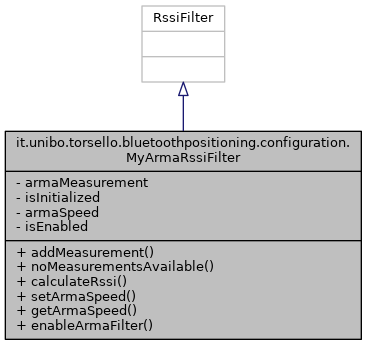
\includegraphics[width=0.6\linewidth]{img/uml/class/classit_1_1unibo_1_1torsello_1_1bluetoothpositioning_1_1configuration_1_1MyArmaRssiFilter__inherit__graph.png}
	\caption{Classe - MyArmaRssiFilter}
\end{figure}

Classe in cui si esegue il filtraggio ARMA spiegato in \ref{ch:filtro_arma}.

\begin{figure}[ph]
	\centering
	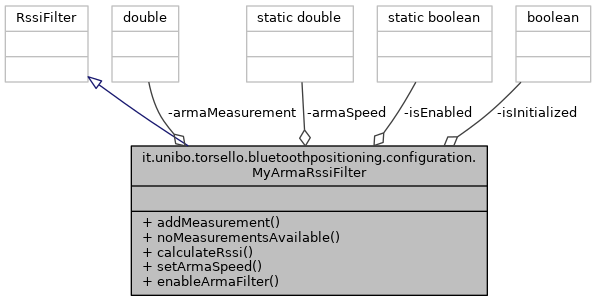
\includegraphics[width=0.65\linewidth]{img/uml/class/classit_1_1unibo_1_1torsello_1_1bluetoothpositioning_1_1configuration_1_1MyArmaRssiFilter__coll__graph.png}
	\caption{Collaborazione - MyArmaRssiFilter}
\end{figure}

\newpage
\section{KFilterBuildertFragment}
Classe di supporto per la creazione di un \texttt{KFilter}. Il suo scopo è inizializzare tale oggetto con dei parametri passati al costruttore.
\begin{figure}[ph]
	\centering
	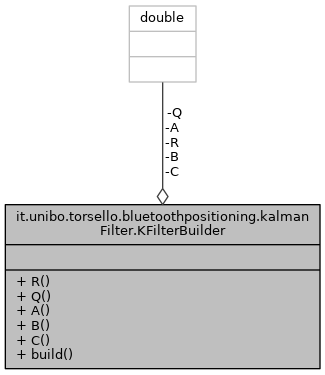
\includegraphics[width=0.6\linewidth]{img/uml/class/classit_1_1unibo_1_1torsello_1_1bluetoothpositioning_1_1kalmanFilter_1_1KFilterBuilder__coll__graph.png}
	\caption{Collaborazione - KFilterBuildertFragment}
\end{figure}

\newpage
\section{KFilter}

Classe per l'implementazione del filtro di Kalman. Il suo funzionamento viene spiegato in \ref{ch:kfilter}.

\begin{figure}[ph]
	\centering
	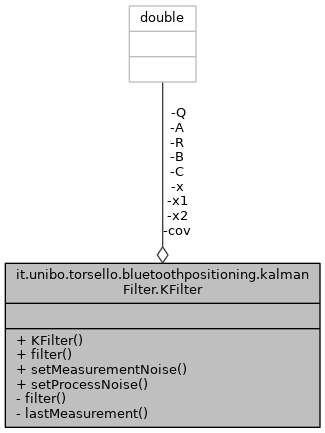
\includegraphics[width=0.6\linewidth]{img/uml/class/classit_1_1unibo_1_1torsello_1_1bluetoothpositioning_1_1kalmanFilter_1_1KFilter__coll__graph.png}
	\caption{Collaborazione - KFilter}
\end{figure}

\newpage
\section{KFilterConstants}
\begin{figure}[ph]
	\centering
	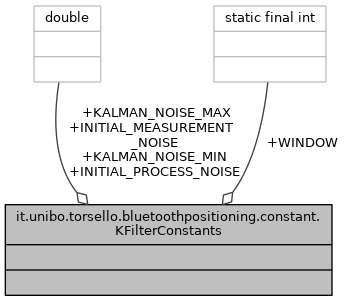
\includegraphics[width=0.6\linewidth]{img/uml/class/classit_1_1unibo_1_1torsello_1_1bluetoothpositioning_1_1constant_1_1KFilterConstants__coll__graph.png}
	\caption{Collaborazione - KFilterConstants}
\end{figure}

\newpage
\section{StatePagerAdapter}
\begin{figure}[ph]
	\centering
	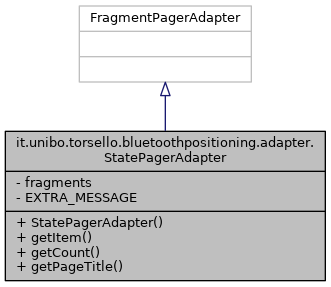
\includegraphics[width=0.5\linewidth]{img/uml/class/classit_1_1unibo_1_1torsello_1_1bluetoothpositioning_1_1adapter_1_1StatePagerAdapter__inherit__graph.png}
	\caption{Classe - StatePagerAdapter}
\end{figure}

Questa classe estende FragmentPagerAdapter per creare un ambiente in cui aggiungere i fragment dei dettagli riguardanti i beacon.

\begin{figure}[ph]
	\centering
	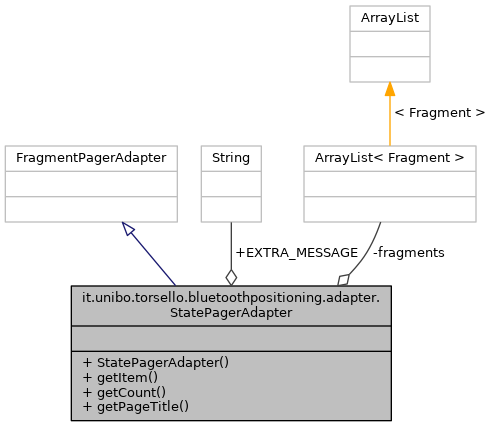
\includegraphics[width=0.75\linewidth]{img/uml/class/classit_1_1unibo_1_1torsello_1_1bluetoothpositioning_1_1adapter_1_1StatePagerAdapter__coll__graph.png}
	\caption{Collaborazione - StatePagerAdapter}
\end{figure}

\newpage
\section{DeviceDetailFragment}
\begin{figure}[ph]
	\centering
	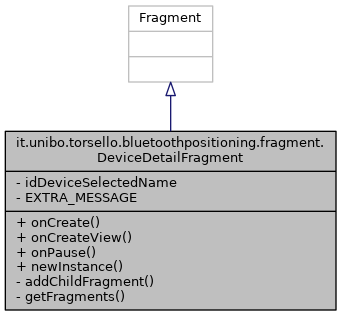
\includegraphics[width=0.5\linewidth]{img/uml/class/classit_1_1unibo_1_1torsello_1_1bluetoothpositioning_1_1fragment_1_1DeviceDetailFragment__inherit__graph.png}
	\caption{Classe - DeviceDetailFragment}
\end{figure}

Classe che istanzia \texttt{StatePagerAdapter} per aggiunge i fragment dei dettagli.

\begin{figure}[ph]
	\centering
	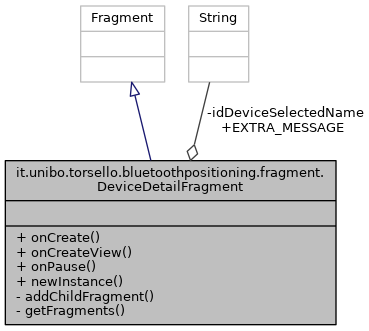
\includegraphics[width=0.7\linewidth]{img/uml/class/classit_1_1unibo_1_1torsello_1_1bluetoothpositioning_1_1fragment_1_1DeviceDetailFragment__coll__graph.png}
	\caption{Collaborazione - DeviceDetailFragment}
\end{figure}

\newpage
\section{CameraFragment}
\begin{figure}[ph]
	\centering
	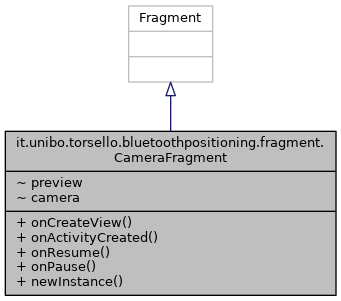
\includegraphics[width=0.5\linewidth]{img/uml/class/classit_1_1unibo_1_1torsello_1_1bluetoothpositioning_1_1fragment_1_1CameraFragment__inherit__graph.png}
	\caption{Classe - CameraFragment}
\end{figure}

Classe per implementare una SurfaceView come preview delle fotocamera presente nello smartphone e scattare delle foto (agli iBeacon). Per scattare le foto si è utilizzato un FloatingActionButton, mentre per fare l'autozoom basta cliccare sulla surface stessa.

\begin{figure}[ph]
	\centering
	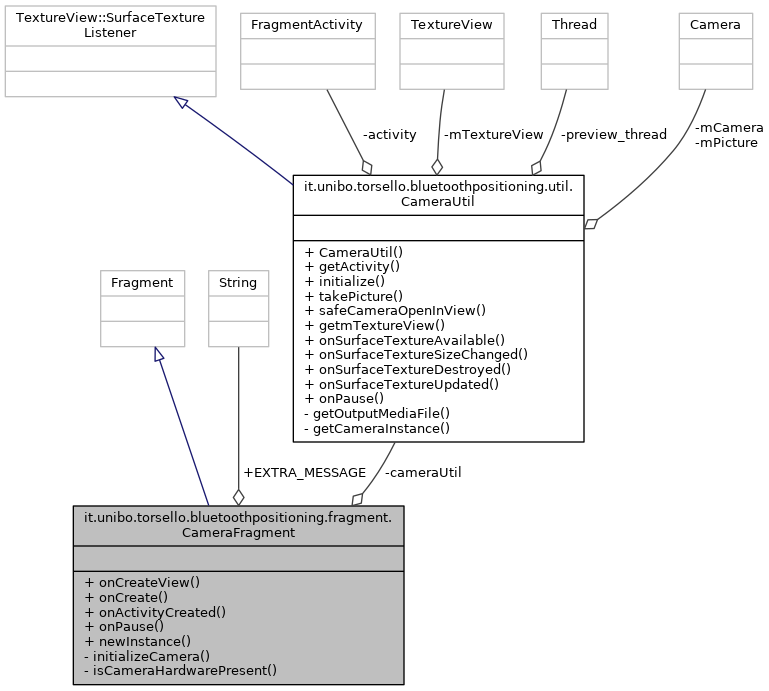
\includegraphics[width=1.7\linewidth, angle=90]{img/uml/class/classit_1_1unibo_1_1torsello_1_1bluetoothpositioning_1_1fragment_1_1CameraFragment__coll__graph.png}
	\caption{Collaborazione - CameraFragment}
\end{figure}

\newpage
\section{CameraPreviewUtil}
\begin{figure}[ph]
	\centering
	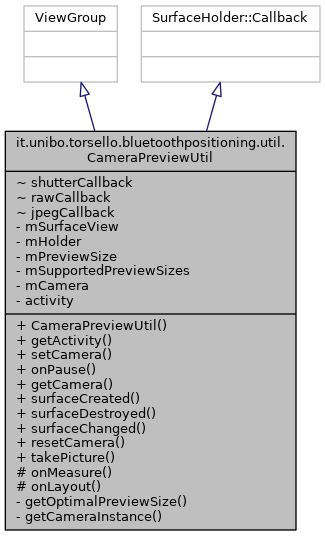
\includegraphics[width=0.5\linewidth]{img/uml/class/classit_1_1unibo_1_1torsello_1_1bluetoothpositioning_1_1util_1_1CameraPreviewUtil__inherit__graph.png}
	\caption{Classe - CameraPreviewUtil}
\end{figure}

Classe che controlla la SurfaceView di preview delle fotocamera e la telecamera stessa. Viene istanziata in \texttt{CameraFragment}.

\begin{figure}[ph]
	\centering
	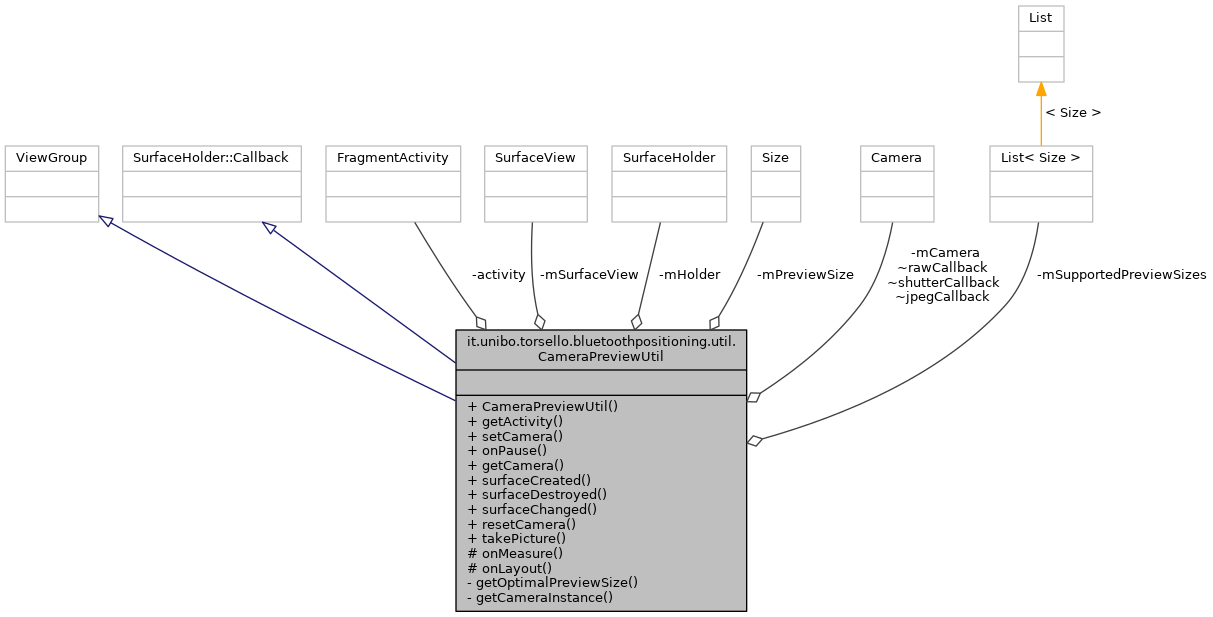
\includegraphics[width=1.5\linewidth,angle=90]{img/uml/class/classit_1_1unibo_1_1torsello_1_1bluetoothpositioning_1_1util_1_1CameraPreviewUtil__coll__graph.png}
	\caption{Collaborazione - CameraPreviewUtil}
\end{figure}

\newpage
\section{SaveImageTask}
\begin{figure}[ph]
	\centering
	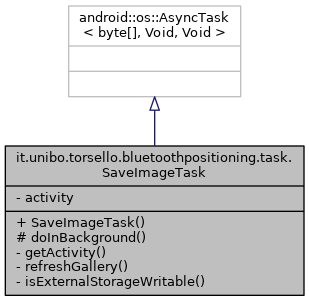
\includegraphics[width=0.5\linewidth]{img/uml/class/classit_1_1unibo_1_1torsello_1_1bluetoothpositioning_1_1task_1_1SaveImageTask__inherit__graph.png}
	\caption{Classe - SaveImageTask}
\end{figure}

Classe che serve a salvare le foto scattate dalla fotocamera. Implementa un AsyncTask per evitare che la GUI di Android si blocchi durante l'elaborazione dell'immagine.

\begin{figure}[ph]
	\centering
	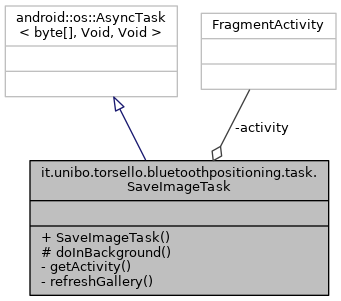
\includegraphics[width=0.5\linewidth]{img/uml/class/classit_1_1unibo_1_1torsello_1_1bluetoothpositioning_1_1task_1_1SaveImageTask__coll__graph.png}
	\caption{Collaborazione - SaveImageTask}
\end{figure}

\newpage
\section{DeviceDetailInner1Fragment}
\begin{figure}[ph]
	\centering
	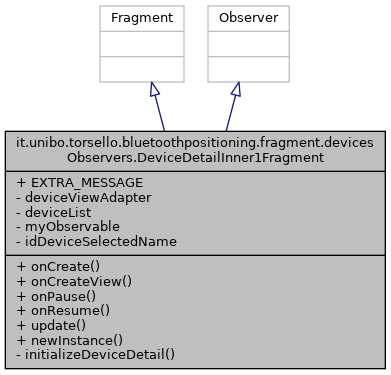
\includegraphics[width=0.5\linewidth]{img/uml/class/classit_1_1unibo_1_1torsello_1_1bluetoothpositioning_1_1fragment_1_1devicesObservers_1_1DeviceDe8362efa0b556f228cc3338a27b7e447c.png}
	\caption{Classe - DeviceDetailInner1Fragment}
\end{figure}

Simile a \ref{ch:device_list}, aggiorna i dati di un solo beacon e visualizza la distanza dall'Arduino. Per la distanza stimata da Arduino si utilizza il fragment \texttt{UsbMeasurementFragment}, istanziato come fragment statico nel file XML.

\begin{figure}[ph]
	\centering
	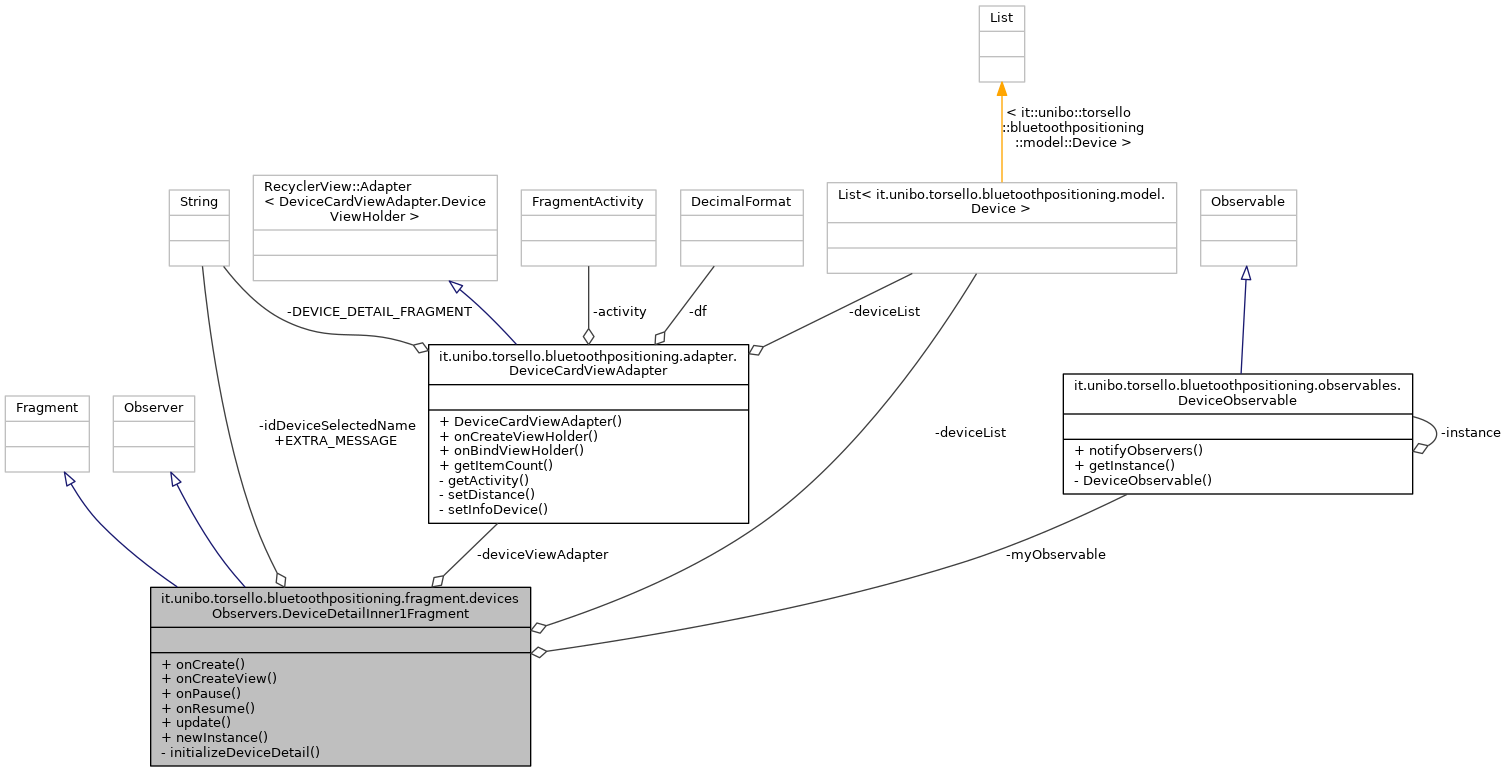
\includegraphics[width=1.8\linewidth,angle=90]{img/uml/class/classit_1_1unibo_1_1torsello_1_1bluetoothpositioning_1_1fragment_1_1devicesObservers_1_1DeviceDetailInner1Fragment__coll__graph.png}
	\caption{Collaborazione - DeviceDetailInner1Fragment}
\end{figure}

\newpage
\section{DeviceDetailInner2Fragment}
\begin{figure}[ph]
	\centering
	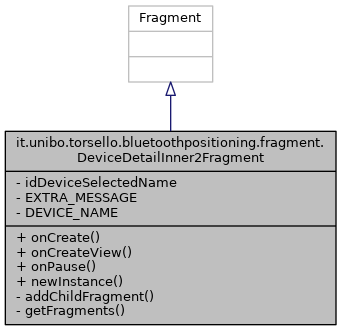
\includegraphics[width=0.5\linewidth]{img/uml/class/classit_1_1unibo_1_1torsello_1_1bluetoothpositioning_1_1fragment_1_1DeviceDetailInner2Fragment__inherit__graph.png}
	\caption{Classe - DeviceDetailInner2Fragment}
\end{figure}

Questa classe estende Fragment per inserire al proprio interno i dettagli dei beacon sotto forma di grafici in real time. L'obiettivo è permettere all'utente di controllare l'evoluzione del sistema e salvare i grafici sotto forma di immagini JPG.

\begin{figure}[ph]
	\centering
	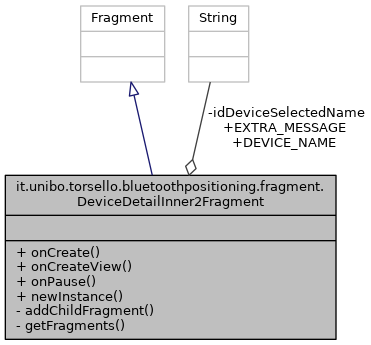
\includegraphics[width=0.55\linewidth]{img/uml/class/classit_1_1unibo_1_1torsello_1_1bluetoothpositioning_1_1fragment_1_1DeviceDetailInner2Fragment__coll__graph.png}
	\caption{Collaborazione - }
\end{figure}

\newpage
\section{DeviceChartFragment}
\begin{figure}[ph]
	\centering
	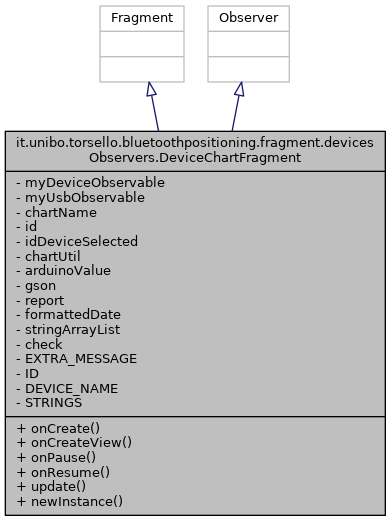
\includegraphics[width=0.5\linewidth]{img/uml/class/classit_1_1unibo_1_1torsello_1_1bluetoothpositioning_1_1fragment_1_1devicesObservers_1_1DeviceChartFragment__inherit__graph.png}
	\caption{Classe - DeviceChartFragment}
\end{figure}

Classe in cui si generano i grafici in realtime. I valori che vengono plottati sono le stime della distanza secondo Arduino e in base ai vari filtri su RSSI.

\begin{figure}[ph]
	\centering
	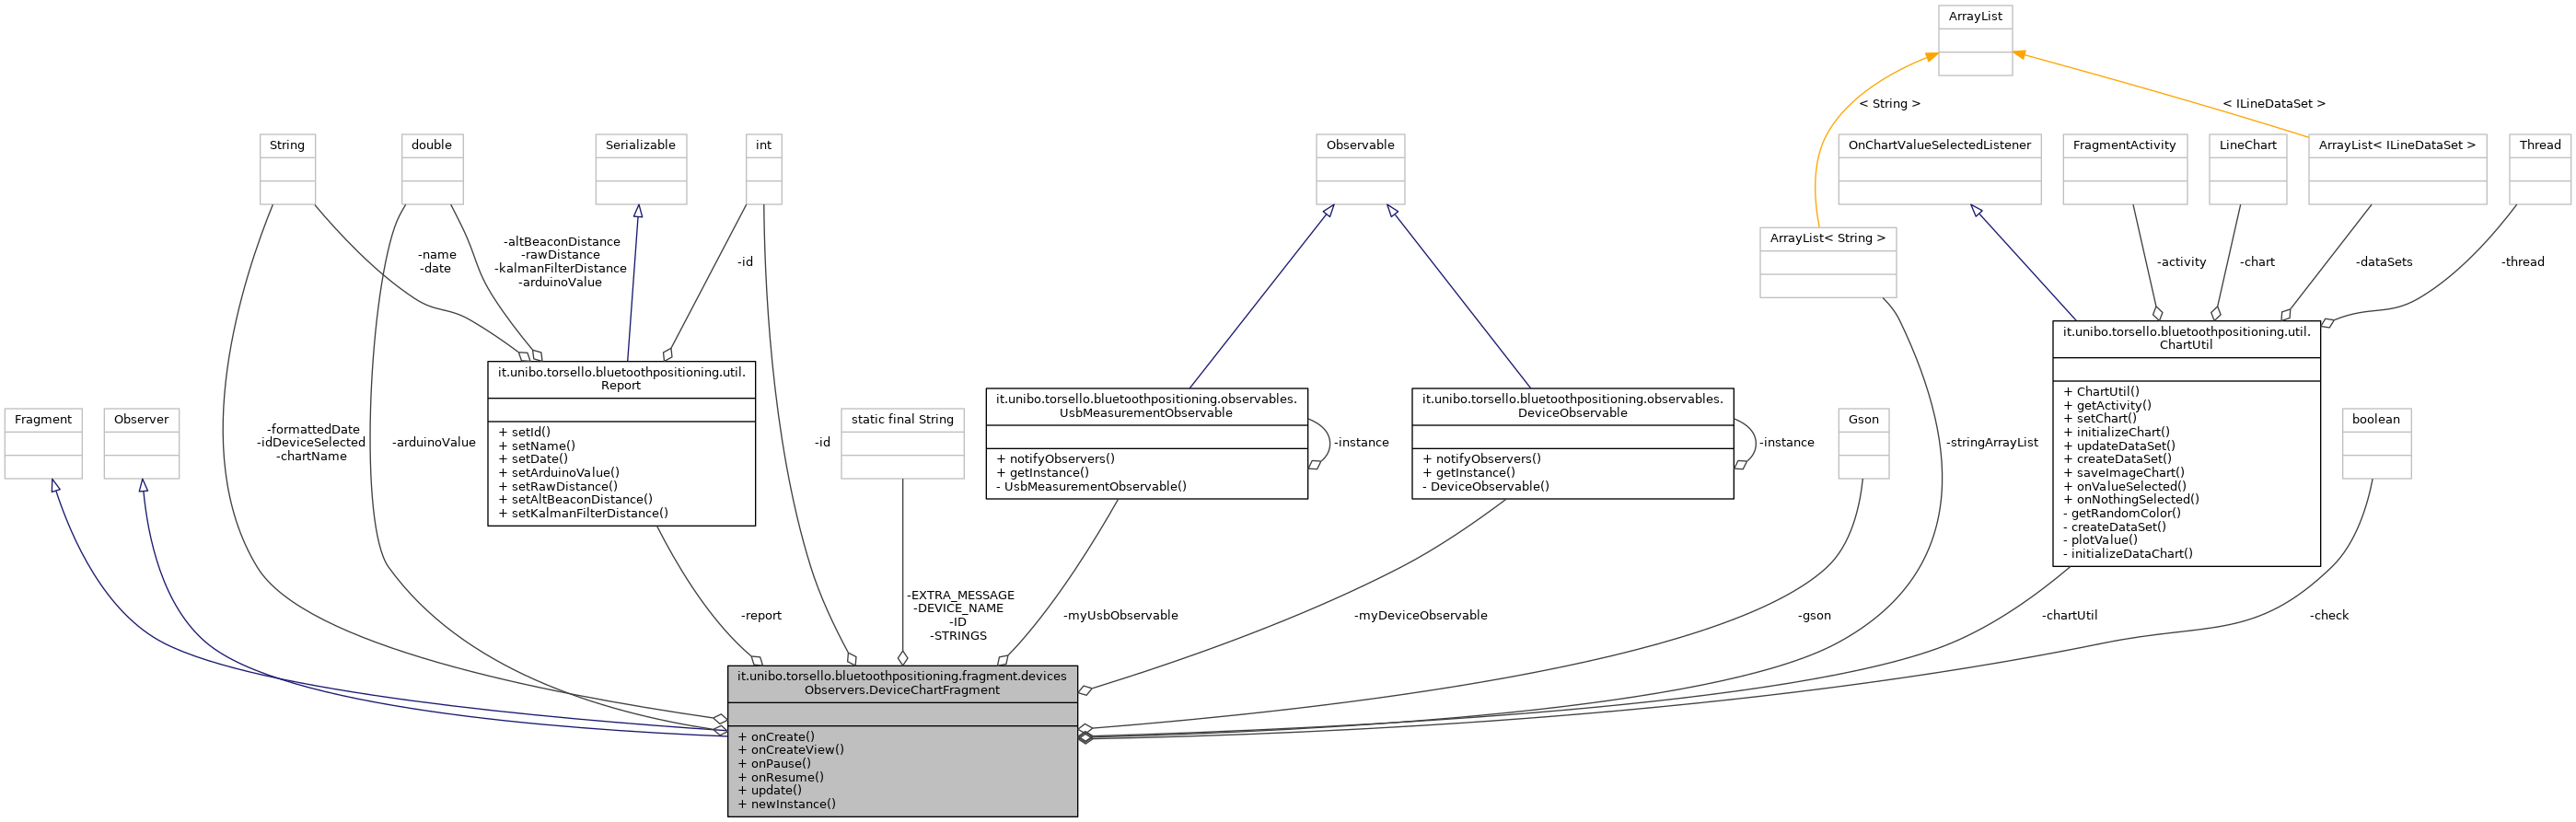
\includegraphics[width=1.8\linewidth,angle=90]{img/uml/class/classit_1_1unibo_1_1torsello_1_1bluetoothpositioning_1_1fragment_1_1devicesObservers_1_1DeviceChartFragment__coll__graph.png}
	\caption{Collaborazione - DeviceChartFragment}
\end{figure}

\newpage
\section{ChartUtil}

Classe per la creazione di grafici in real time. Viene sfuttata da \texttt{DeviceChartFragment} per istanziare un oggetto \texttt{LinearChart} a cui passare le varie distanze stimate via RSSI e USB.
\begin{figure}[ph]
	\centering
	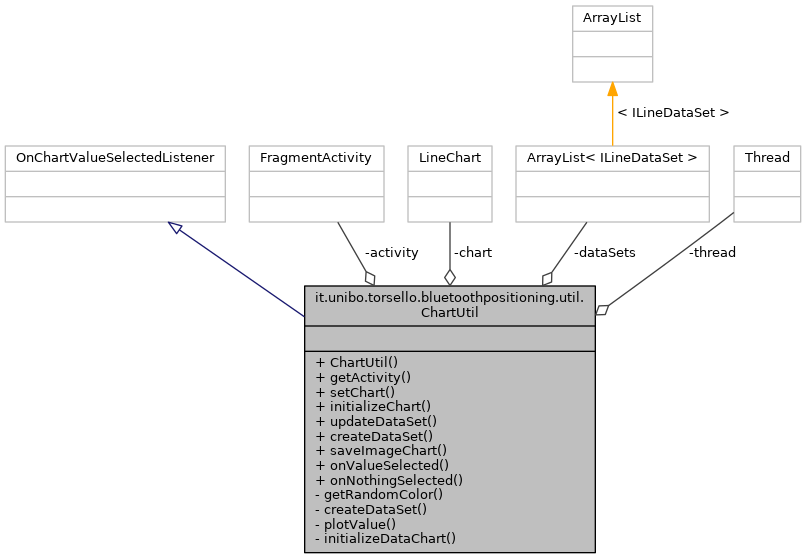
\includegraphics[width=1.2\linewidth]{img/uml/class/classit_1_1unibo_1_1torsello_1_1bluetoothpositioning_1_1util_1_1ChartUtil__coll__graph.png}
	\caption{}
\end{figure}

\newpage
\section{UsbMeasurementFragment}
\begin{figure}[ph]
	\centering
	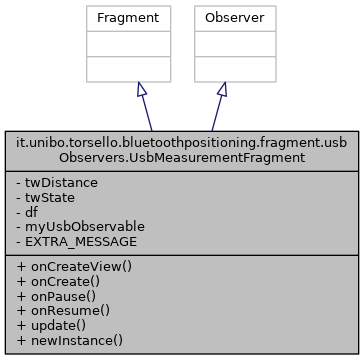
\includegraphics[width=0.5\linewidth]{img/uml/class/classit_1_1unibo_1_1torsello_1_1bluetoothpositioning_1_1fragment_1_1usbObservers_1_1UsbMeasurementFragment__inherit__graph.png}
	\caption{Classe - UsbMeasurementFragment}
\end{figure}

Classe che visualizza su di un fragment i valori di distanza stimati dall'Arduino. Questa visualizzazione viene riutilizzata da sola se si seleziona "Measurement" dal menu a sinistra che nei dettagli. Nel caso dei dettagli il fragment è istanziato come statico dal file XML come segue:

\begin{lstlisting}[language=XML]
<android.support.v7.widget.CardView android:layout_width="match_parent"	android:layout_height="wrap_content" android:layout_margin="@dimen/card_margin">

	<fragment android:layout_width="match_parent" android:layout_height="wrap_content" android:name="it.unibo.torsello.bluetoothpositioning
	.fragment.usbObservers.UsbMeasurementFragment" android:id="@+id/usbArduino" tools:layout="@layout/fragment_usb_measurement" />
</android.support.v7.widget.CardView>
\end{lstlisting}

\begin{figure}[ph]
	\centering
	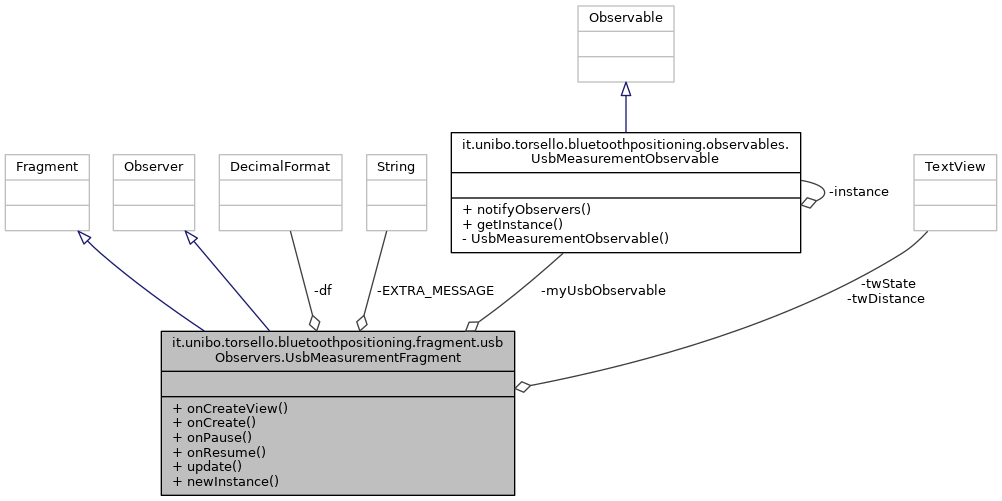
\includegraphics[width=1.6\linewidth,angle=90]{img/uml/class/classit_1_1unibo_1_1torsello_1_1bluetoothpositioning_1_1fragment_1_1usbObservers_1_1UsbMeasurementFragment__coll__graph.png}
	\caption{Collaborazione - UsbMeasurementFragment}
\end{figure}

\newpage
\section{UsbUtil}

Classe che permette di comunicare con la porta USB dello smartphone e in questo caso di ricevere i dati della distanza stimata da Arduino. 

Per inizializzare la comunicazione su USB si utilizza il metodo \texttt{initializeUsb()}
\subsubsection{Metodo initializeUsb()}
\begin{lstlisting}[language=Java]
private void initializeUsb() {
	
	// Find all available drivers from attached devices.
	UsbManager usbManager = (UsbManager) getActivity().getSystemService(Context.USB_SERVICE);
	List<UsbSerialDriver> availableDrivers = UsbSerialProber.getDefaultProber()
		.findAllDrivers(usbManager);
		
	if (!availableDrivers.isEmpty()) {
		
		// Open a connection to the first available driver.
		UsbSerialDriver driver = availableDrivers.get(0);
		
		if (usbManager.hasPermission(driver.getDevice())) {
			if (usbManager.openDevice(driver.getDevice()) != null) {
				// Read some data! Most have just one port (port 0).
				port = driver.getPorts().get(0);
			}
		} else {
			Intent startIntent = new Intent(getActivity(), getClass());
			PendingIntent pendingIntent =
				PendingIntent.getService(getActivity(), 0, startIntent, 0);
			usbManager.requestPermission(driver.getDevice(), pendingIntent);
		}
		
		if (port != null) {
			
			UsbDeviceConnection connection = 
				usbManager.openDevice(port.getDriver()
					.getDevice());
			
			if (connection != null) {
				try {
					port.open(connection);
					port.setParameters(BOUND_RATE, UsbSerialPort.DATABITS_8,
					UsbSerialPort.STOPBITS_1, UsbSerialPort.PARITY_NONE);
				} catch (IOException e) {
					myUsbObservable.notifyObservers(getActivity()
						.getString(R.string.error_opening_device)
						+ " " + e.getMessage());
					myUsbObservable.notifyObservers(false);
					closePort();
					return;
				}
				
				stopIoManager();
				startIoManager();
			}
		}
	}
}
\end{lstlisting}

\begin{figure}[ph]
	\centering
	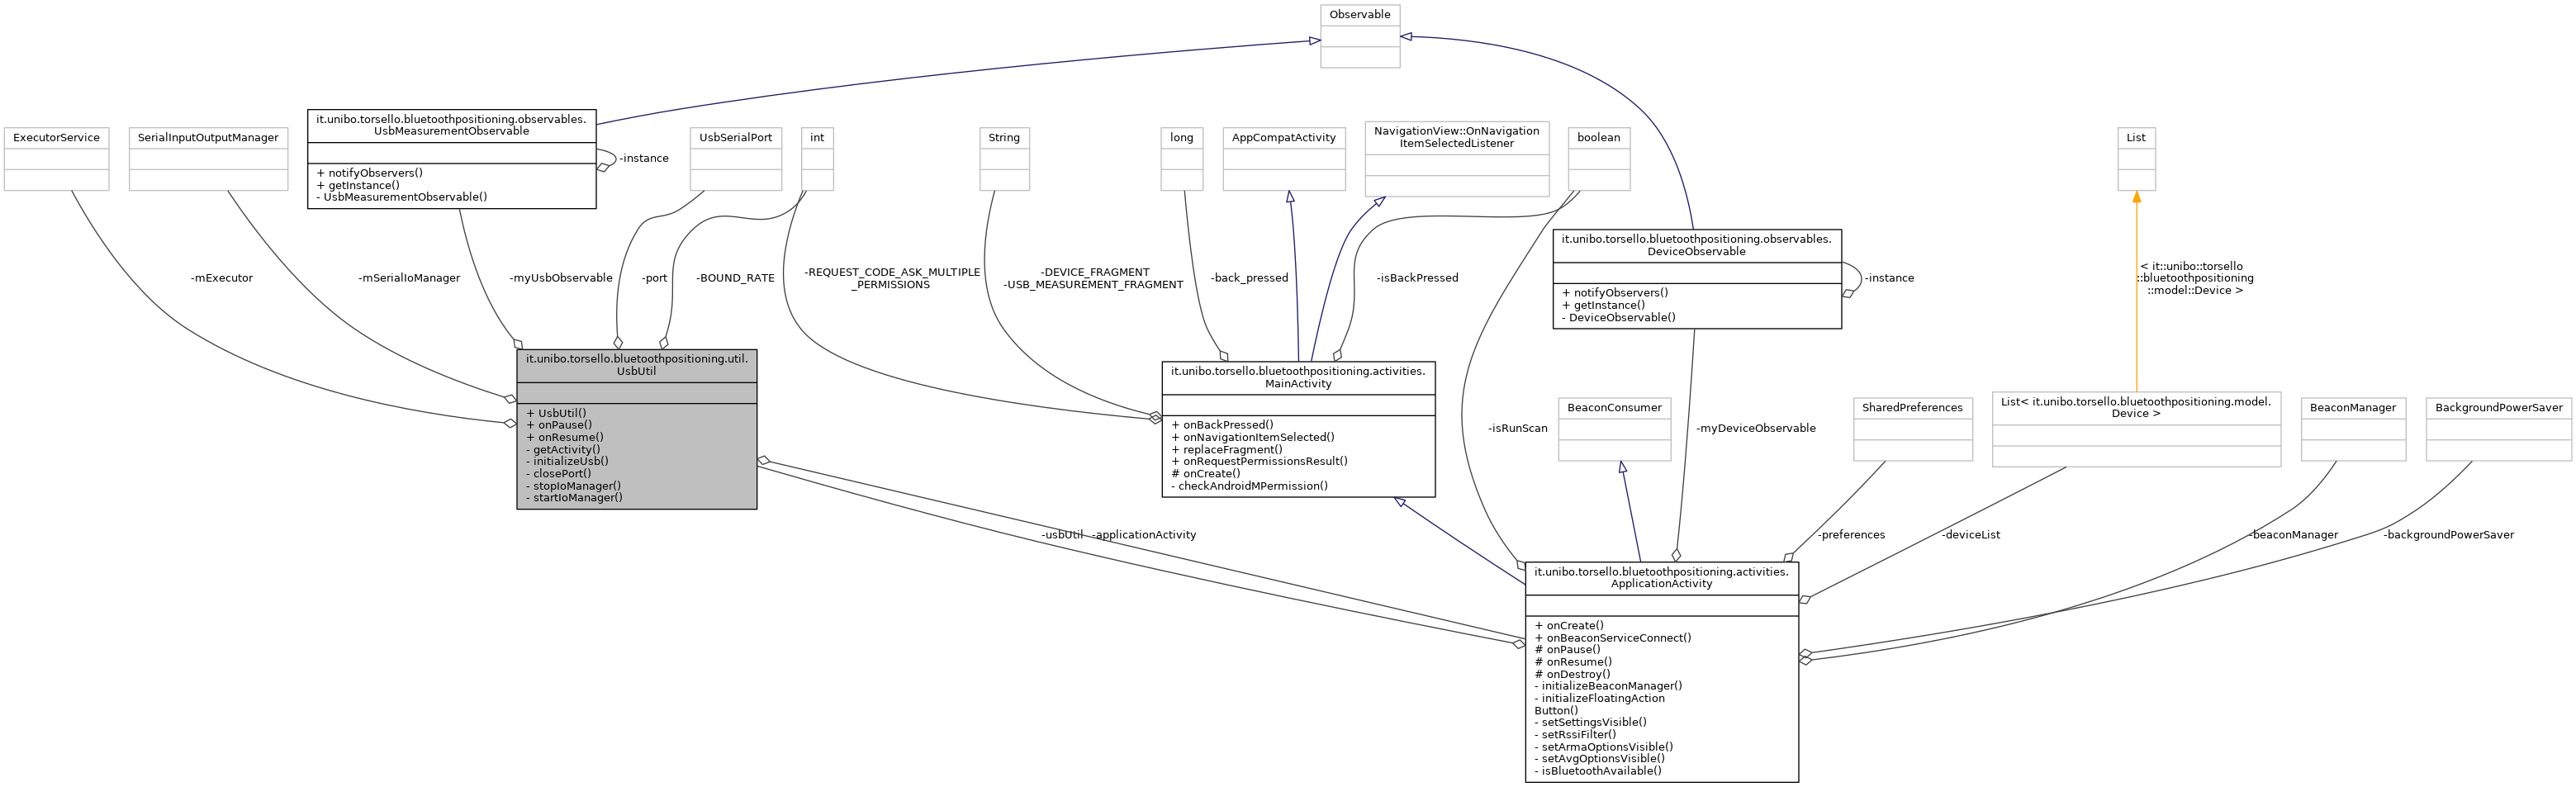
\includegraphics[width=1.85\linewidth,angle=90]{img/uml/class/classit_1_1unibo_1_1torsello_1_1bluetoothpositioning_1_1util_1_1UsbUtil__coll__graph.png}
	\caption{Collaborazione - UsbUtil}
\end{figure}

\newpage
\section{UsbMeasurementObservable}
\begin{figure}[ph]
	\centering
	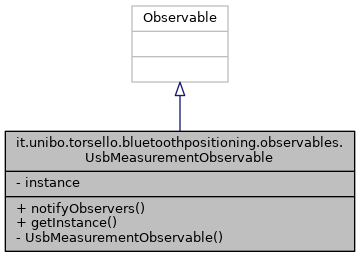
\includegraphics[width=0.6\linewidth]{img/uml/class/classit_1_1unibo_1_1torsello_1_1bluetoothpositioning_1_1observables_1_1UsbMeasurementObservable__inherit__graph.png}
	\caption{Classe - UsbMeasurementObservable}
\end{figure}

Classe Observable che emette le distanze stimate da Arduino a tutti gli Observer a lui registrati.

\begin{figure}[ph]
	\centering
	\includegraphics[width=0.8\linewidth]{img/uml/class/classit_1_1unibo_1_1torsello_1_1bluetoothpositioning_1_1observables_1_1UsbMeasurementObservable__coll__graph.png}
	\caption{Collaborazione - UsbMeasurementObservable}
\end{figure}

\newpage
\section{FABBehavior}
\begin{figure}[ph]
	\centering
	\includegraphics[width=0.6\linewidth]{img/uml/class/classit_1_1unibo_1_1torsello_1_1bluetoothpositioning_1_1extra_1_1FABBehavior__inherit__graph.png}
	\caption{Classe - FABBehavior}
\end{figure}

Classe che amplia il comportamento del FloatingActionButton in basso a destra, facendolo scomparire per un secondo quando una RecyclerView viene scrollata in alto o in basso.
Per funzionare si è dovuto modificare il file XML in cui il FAB è inserito con la regola \texttt{app:layout\_behavior=".extra.FABBehavior"}.
%	\chapter{Gerarchia delle classi}

\section{MainActivity}
\begin{figure}[ph]
	\centering
	\includegraphics[width=0.40\linewidth]{img/uml/class/classit_1_1unibo_1_1torsello_1_1bluetoothpositioning_1_1activities_1_1MainActivity__inherit__graph.png}
	\caption{Classe - MainActivity}
\end{figure}
La classe \texttt{Main} viene istanziata per prima all'avvio dell'app. Serve ad inizializzare gli oggetti grafici, controllare la compatibilità con Android 5.0+ e rimpiazzare i fragment da visualizzare selezionati dal menu a sinistra.

\begin{figure}[ph]
	\centering
	\includegraphics[width=1.8\linewidth,angle=90]{img/uml/class/classit_1_1unibo_1_1torsello_1_1bluetoothpositioning_1_1activities_1_1MainActivity__coll__graph.png}
	\caption{Collaborazione - MainActivity}
\end{figure}

\newpage
\section{ApplicationActivity}
\begin{figure}[ph]
	\centering
	\includegraphics[width=0.7\linewidth]{img/uml/class/classit_1_1unibo_1_1torsello_1_1bluetoothpositioning_1_1activities_1_1ApplicationActivity__inherit__graph.png}
	\caption{Classe - ApplicationActivity}
\end{figure}

Questa classe è una parte fondamentale del progetto. Qui si istanzia e controlla l'oggetto \texttt{BeaconManager} responsabile dello scanning su BT e quindi si ricevono le informazioni dei dispositivi vicini.

Alla ricezione dei dati, questi vengono spediti al \texttt{DeviceObservable} a cui tutti gli Observer interessati si registreranno in modo da ottenere tutti lo stesso valore aggiornato.

\begin{figure}[ph]
	\centering
	\includegraphics[width=1.9\linewidth, angle=90]{img/uml/class/classit_1_1unibo_1_1torsello_1_1bluetoothpositioning_1_1activities_1_1ApplicationActivity__coll__graph.png}
	\caption{Collaborazione - ApplicationActivity}
\end{figure}

\newpage
\section{Device}
\begin{figure}[ph]
	\centering
	\includegraphics[width=0.9\linewidth]{img/uml/class/classit_1_1unibo_1_1torsello_1_1bluetoothpositioning_1_1model_1_1Device__coll__graph.png}
	\caption{Collaborazione - Device}
\end{figure}

Classe che modella la definizione di dispositivo Bluetooth BLE nel sistema. Alcuni dei dati presenti nella classe sono inizializzati alla creazione che avviene nella classe \texttt{DeviceConstants}, altri sono invece calcolati durante l'esecuzione, come la stima della distanza da parte dei vari filtri.

\newpage
\section{DeviceConstants}
\begin{figure}[ph]
	\centering
	\includegraphics[width=0.7\linewidth]{img/uml/class/classit_1_1unibo_1_1torsello_1_1bluetoothpositioning_1_1constant_1_1DeviceConstants__coll__graph.png}
	\caption{Collaborazione - DeviceConstants}
\end{figure}

Classe che modella ed inizializza i dispositivi sotto forma di oggetto \texttt{Device}. Al suo interno è presente una \texttt{Map} in cui sono indicati i soli ed unici dispositivi che saranno riconosciuti dal sistema.

\newpage
\section{DeviceObservable}
\begin{figure}[ph]
	\centering
	\includegraphics[width=0.7\linewidth]{img/uml/class/classit_1_1unibo_1_1torsello_1_1bluetoothpositioning_1_1observables_1_1DeviceObservable__inherit__graph.png}
	\caption{Classe - DeviceObservable}
\end{figure}

Lo scopo di questa classe è creare un Observable che notifichi a tutti gli Observer registrati l'oggetto list con tutti gli update dei dispositivi scansionati. Questa lista viene aggiornata nella classe \texttt{ApplicationActivity} nel metodo \texttt{onBeaconServiceConnect}

\newpage
\section{Estimation}
\begin{figure}[ph]
	\centering
	\includegraphics[width=1.2\linewidth]{img/uml/class/classit_1_1unibo_1_1torsello_1_1bluetoothpositioning_1_1distanceEstimation_1_1Estimation__coll__graph.png}
	\caption{Collaborazione - Estimation}
\end{figure}

\newpage
\section{SettingsFragment}
\begin{figure}[ph]
	\centering
	\includegraphics[width=0.5\linewidth]{img/uml/class/classit_1_1unibo_1_1torsello_1_1bluetoothpositioning_1_1fragment_1_1SettingsFragment__inherit__graph.png}
	\caption{Classe - SettingsFragment}
\end{figure}

Classe che implementa Fragment per creare una vista disposta in un menu a destra. Il suo scopo è permettere all'utente di interagire con l'app e con il sistema fisico in cui ci si esegue la stima modificando dei semplici parametri.

\newpage
Nel particolare si usa l'oggetto \texttt{SharedPreferences} per salvare le impostazioni utilizzate. Nel caso in cui l'app fosse chiusa, le impostazioni salvate precedentemente vengono reimpostate come se l'app non fosse mai stata terminata.

\begin{figure}[ph]
	\centering
	\includegraphics[width=0.8\linewidth]{img/uml/class/classit_1_1unibo_1_1torsello_1_1bluetoothpositioning_1_1fragment_1_1SettingsFragment__coll__graph.png}
	\caption{Collaborazione - SettingsFragment}
\end{figure}

\newpage
\section{SettingConstants}

Classe in cui si settano le costanti relative ai settaggi. Tali costanti sono intese come chiavi per risalire alle impostazioni scelte dall'utente, come ad esempio il filtro o l'ordinamento dei dispositivi trovati.
\begin{figure}[ph]
	\centering
	\includegraphics[width=0.5\linewidth]{img/uml/class/classit_1_1unibo_1_1torsello_1_1bluetoothpositioning_1_1constant_1_1SettingConstants__coll__graph.png}
	\caption{Collaborazione - SettingConstants}
\end{figure}

\newpage
\section{DeviceListFragment}\label{ch:device_list}
\begin{figure}[ph]
	\centering
	\includegraphics[width=0.5\linewidth]{img/uml/class/classit_1_1unibo_1_1torsello_1_1bluetoothpositioning_1_1fragment_1_1devicesObservers_1_1DeviceListFragment__inherit__graph.png}
	\caption{Classe - DeviceListFragment}
\end{figure}

Classe che aggiorna la lista dei dispositivi con le nuove informazioni ricevute dal metodo \texttt{update(...)}, \textit{override} della classe Observer.
\begin{lstlisting}[language=Java]
@Override
publilc void update(Observable o, Object arg) {
	
	if (arg instanceof List) {
		
		if (!deviceList.isEmpty()) {
			deviceList.clear();
		}
		
		List<Device> devices = (List<Device>) arg;
		
		// optional sorting
		Collections.sort(devices, new Comparator<Device>() {
			public int compare(Device b1, Device b2) {
				int sorting = preferences
					.getInt(SettingConstants.DISTANCE_SORTING, 0);
				switch (sorting) {
					case 0:
					case R.id.radioButton_default_sorting:
					return Double.compare(b1.getIndex(), b2.getIndex());
					case R.id.radioButton_color_sorting:
					return Double.compare(b1.getColor(), b2.getColor());
					case R.id.radioButton_distance_sorting:
					return Double.compare(b1.getKalmanFilterDistance(), b2.getKalmanFilterDistance());
				} // default sorting (a good basic ordering for the other options)
				return Double.compare(b1.getIndex(), 
						b2.getIndex());
			}
		});
		
		deviceList.addAll(devices);
		deviceViewAdapter.notifyDataSetChanged();
	}
}
\end{lstlisting}

Nel dettaglio si aggiorna la lista in base alle preferenze impostate in \texttt{Settings}.

\begin{figure}[ph]
	\centering
	\includegraphics[width=1.9\linewidth,angle=90]{img/uml/class/classit_1_1unibo_1_1torsello_1_1bluetoothpositioning_1_1fragment_1_1devicesObservers_1_1DeviceListFragment__coll__graph.png}
	\caption{Collaborazione - DeviceListFragment}
\end{figure}

\newpage
\section{DeviceCardViewAdapter}
\begin{figure}[ph]
	\centering
	\includegraphics[width=0.5\linewidth]{img/uml/class/classit_1_1unibo_1_1torsello_1_1bluetoothpositioning_1_1adapter_1_1DeviceCardViewAdapter__inherit__graph.png}
	\caption{Classe - DeviceCardViewAdapter}
\end{figure}

Classe responsabile della visualizzazione delle nuove informazioni a schermo. Qui si gestiscono gli elementi grafici da fare vedere o nascondere (valori testuali o immagini) nella RecyclerView.

Viene utilizzata nella schermata principale e nel fragment dei dettagli.

\begin{figure}[ph]
	\centering
	\includegraphics[width=1.5\linewidth,angle=90]{img/uml/class/classit_1_1unibo_1_1torsello_1_1bluetoothpositioning_1_1adapter_1_1DeviceCardViewAdapter__coll__graph.png}
	\caption{Collaborazione - DeviceCardViewAdapter}
\end{figure}

\newpage
\section{DeviceViewHolder}
\begin{figure}[ph]
	\centering
	\includegraphics[width=0.5\linewidth]{img/uml/class/classit_1_1unibo_1_1torsello_1_1bluetoothpositioning_1_1adapter_1_1DeviceCardViewAdapter_1_1DeviceViewHolder__inherit__graph.png}
	\caption{Classe - DeviceViewHolder}
\end{figure}

Classe che serve ad inizializzare i vari oggetti grafici da visualizzare nel RecyclerView, risparmiando memoria.

\begin{figure}[ph]
	\centering
	\includegraphics[width=1.5\linewidth,angle=90]{img/uml/class/classit_1_1unibo_1_1torsello_1_1bluetoothpositioning_1_1adapter_1_1DeviceCardViewAdapter_1_1DeviceViewHolder__coll__graph.png}
	\caption{Collaborazione - DeviceViewHolder}
\end{figure}

\newpage
\section{MyArmaRssiFilter}
\begin{figure}[ph]
	\centering
	\includegraphics[width=0.6\linewidth]{img/uml/class/classit_1_1unibo_1_1torsello_1_1bluetoothpositioning_1_1configuration_1_1MyArmaRssiFilter__inherit__graph.png}
	\caption{Classe - MyArmaRssiFilter}
\end{figure}

Classe in cui si esegue il filtraggio ARMA spiegato in \ref{ch:filtro_arma}.

\begin{figure}[ph]
	\centering
	\includegraphics[width=0.65\linewidth]{img/uml/class/classit_1_1unibo_1_1torsello_1_1bluetoothpositioning_1_1configuration_1_1MyArmaRssiFilter__coll__graph.png}
	\caption{Collaborazione - MyArmaRssiFilter}
\end{figure}

\newpage
\section{KFilterBuildertFragment}
Classe di supporto per la creazione di un \texttt{KFilter}. Il suo scopo è inizializzare tale oggetto con dei parametri passati al costruttore.
\begin{figure}[ph]
	\centering
	\includegraphics[width=0.6\linewidth]{img/uml/class/classit_1_1unibo_1_1torsello_1_1bluetoothpositioning_1_1kalmanFilter_1_1KFilterBuilder__coll__graph.png}
	\caption{Collaborazione - KFilterBuildertFragment}
\end{figure}

\newpage
\section{KFilter}

Classe per l'implementazione del filtro di Kalman. Il suo funzionamento viene spiegato in \ref{ch:kfilter}.

\begin{figure}[ph]
	\centering
	\includegraphics[width=0.6\linewidth]{img/uml/class/classit_1_1unibo_1_1torsello_1_1bluetoothpositioning_1_1kalmanFilter_1_1KFilter__coll__graph.png}
	\caption{Collaborazione - KFilter}
\end{figure}

\newpage
\section{KFilterConstants}
\begin{figure}[ph]
	\centering
	\includegraphics[width=0.6\linewidth]{img/uml/class/classit_1_1unibo_1_1torsello_1_1bluetoothpositioning_1_1constant_1_1KFilterConstants__coll__graph.png}
	\caption{Collaborazione - KFilterConstants}
\end{figure}

\newpage
\section{StatePagerAdapter}
\begin{figure}[ph]
	\centering
	\includegraphics[width=0.5\linewidth]{img/uml/class/classit_1_1unibo_1_1torsello_1_1bluetoothpositioning_1_1adapter_1_1StatePagerAdapter__inherit__graph.png}
	\caption{Classe - StatePagerAdapter}
\end{figure}

Questa classe estende FragmentPagerAdapter per creare un ambiente in cui aggiungere i fragment dei dettagli riguardanti i beacon.

\begin{figure}[ph]
	\centering
	\includegraphics[width=0.75\linewidth]{img/uml/class/classit_1_1unibo_1_1torsello_1_1bluetoothpositioning_1_1adapter_1_1StatePagerAdapter__coll__graph.png}
	\caption{Collaborazione - StatePagerAdapter}
\end{figure}

\newpage
\section{DeviceDetailFragment}
\begin{figure}[ph]
	\centering
	\includegraphics[width=0.5\linewidth]{img/uml/class/classit_1_1unibo_1_1torsello_1_1bluetoothpositioning_1_1fragment_1_1DeviceDetailFragment__inherit__graph.png}
	\caption{Classe - DeviceDetailFragment}
\end{figure}

Classe che istanzia \texttt{StatePagerAdapter} per aggiunge i fragment dei dettagli.

\begin{figure}[ph]
	\centering
	\includegraphics[width=0.7\linewidth]{img/uml/class/classit_1_1unibo_1_1torsello_1_1bluetoothpositioning_1_1fragment_1_1DeviceDetailFragment__coll__graph.png}
	\caption{Collaborazione - DeviceDetailFragment}
\end{figure}

\newpage
\section{CameraFragment}
\begin{figure}[ph]
	\centering
	\includegraphics[width=0.5\linewidth]{img/uml/class/classit_1_1unibo_1_1torsello_1_1bluetoothpositioning_1_1fragment_1_1CameraFragment__inherit__graph.png}
	\caption{Classe - CameraFragment}
\end{figure}

Classe per implementare una SurfaceView come preview delle fotocamera presente nello smartphone e scattare delle foto (agli iBeacon). Per scattare le foto si è utilizzato un FloatingActionButton, mentre per fare l'autozoom basta cliccare sulla surface stessa.

\begin{figure}[ph]
	\centering
	\includegraphics[width=1.7\linewidth, angle=90]{img/uml/class/classit_1_1unibo_1_1torsello_1_1bluetoothpositioning_1_1fragment_1_1CameraFragment__coll__graph.png}
	\caption{Collaborazione - CameraFragment}
\end{figure}

\newpage
\section{CameraPreviewUtil}
\begin{figure}[ph]
	\centering
	\includegraphics[width=0.5\linewidth]{img/uml/class/classit_1_1unibo_1_1torsello_1_1bluetoothpositioning_1_1util_1_1CameraPreviewUtil__inherit__graph.png}
	\caption{Classe - CameraPreviewUtil}
\end{figure}

Classe che controlla la SurfaceView di preview delle fotocamera e la telecamera stessa. Viene istanziata in \texttt{CameraFragment}.

\begin{figure}[ph]
	\centering
	\includegraphics[width=1.5\linewidth,angle=90]{img/uml/class/classit_1_1unibo_1_1torsello_1_1bluetoothpositioning_1_1util_1_1CameraPreviewUtil__coll__graph.png}
	\caption{Collaborazione - CameraPreviewUtil}
\end{figure}

\newpage
\section{SaveImageTask}
\begin{figure}[ph]
	\centering
	\includegraphics[width=0.5\linewidth]{img/uml/class/classit_1_1unibo_1_1torsello_1_1bluetoothpositioning_1_1task_1_1SaveImageTask__inherit__graph.png}
	\caption{Classe - SaveImageTask}
\end{figure}

Classe che serve a salvare le foto scattate dalla fotocamera. Implementa un AsyncTask per evitare che la GUI di Android si blocchi durante l'elaborazione dell'immagine.

\begin{figure}[ph]
	\centering
	\includegraphics[width=0.5\linewidth]{img/uml/class/classit_1_1unibo_1_1torsello_1_1bluetoothpositioning_1_1task_1_1SaveImageTask__coll__graph.png}
	\caption{Collaborazione - SaveImageTask}
\end{figure}

\newpage
\section{DeviceDetailInner1Fragment}
\begin{figure}[ph]
	\centering
	\includegraphics[width=0.5\linewidth]{img/uml/class/classit_1_1unibo_1_1torsello_1_1bluetoothpositioning_1_1fragment_1_1devicesObservers_1_1DeviceDe8362efa0b556f228cc3338a27b7e447c.png}
	\caption{Classe - DeviceDetailInner1Fragment}
\end{figure}

Simile a \ref{ch:device_list}, aggiorna i dati di un solo beacon e visualizza la distanza dall'Arduino. Per la distanza stimata da Arduino si utilizza il fragment \texttt{UsbMeasurementFragment}, istanziato come fragment statico nel file XML.

\begin{figure}[ph]
	\centering
	\includegraphics[width=1.8\linewidth,angle=90]{img/uml/class/classit_1_1unibo_1_1torsello_1_1bluetoothpositioning_1_1fragment_1_1devicesObservers_1_1DeviceDetailInner1Fragment__coll__graph.png}
	\caption{Collaborazione - DeviceDetailInner1Fragment}
\end{figure}

\newpage
\section{DeviceDetailInner2Fragment}
\begin{figure}[ph]
	\centering
	\includegraphics[width=0.5\linewidth]{img/uml/class/classit_1_1unibo_1_1torsello_1_1bluetoothpositioning_1_1fragment_1_1DeviceDetailInner2Fragment__inherit__graph.png}
	\caption{Classe - DeviceDetailInner2Fragment}
\end{figure}

Questa classe estende Fragment per inserire al proprio interno i dettagli dei beacon sotto forma di grafici in real time. L'obiettivo è permettere all'utente di controllare l'evoluzione del sistema e salvare i grafici sotto forma di immagini JPG.

\begin{figure}[ph]
	\centering
	\includegraphics[width=0.55\linewidth]{img/uml/class/classit_1_1unibo_1_1torsello_1_1bluetoothpositioning_1_1fragment_1_1DeviceDetailInner2Fragment__coll__graph.png}
	\caption{Collaborazione - }
\end{figure}

\newpage
\section{DeviceChartFragment}
\begin{figure}[ph]
	\centering
	\includegraphics[width=0.5\linewidth]{img/uml/class/classit_1_1unibo_1_1torsello_1_1bluetoothpositioning_1_1fragment_1_1devicesObservers_1_1DeviceChartFragment__inherit__graph.png}
	\caption{Classe - DeviceChartFragment}
\end{figure}

Classe in cui si generano i grafici in realtime. I valori che vengono plottati sono le stime della distanza secondo Arduino e in base ai vari filtri su RSSI.

\begin{figure}[ph]
	\centering
	\includegraphics[width=1.8\linewidth,angle=90]{img/uml/class/classit_1_1unibo_1_1torsello_1_1bluetoothpositioning_1_1fragment_1_1devicesObservers_1_1DeviceChartFragment__coll__graph.png}
	\caption{Collaborazione - DeviceChartFragment}
\end{figure}

\newpage
\section{ChartUtil}

Classe per la creazione di grafici in real time. Viene sfuttata da \texttt{DeviceChartFragment} per istanziare un oggetto \texttt{LinearChart} a cui passare le varie distanze stimate via RSSI e USB.
\begin{figure}[ph]
	\centering
	\includegraphics[width=1.2\linewidth]{img/uml/class/classit_1_1unibo_1_1torsello_1_1bluetoothpositioning_1_1util_1_1ChartUtil__coll__graph.png}
	\caption{}
\end{figure}

\newpage
\section{UsbMeasurementFragment}
\begin{figure}[ph]
	\centering
	\includegraphics[width=0.5\linewidth]{img/uml/class/classit_1_1unibo_1_1torsello_1_1bluetoothpositioning_1_1fragment_1_1usbObservers_1_1UsbMeasurementFragment__inherit__graph.png}
	\caption{Classe - UsbMeasurementFragment}
\end{figure}

Classe che visualizza su di un fragment i valori di distanza stimati dall'Arduino. Questa visualizzazione viene riutilizzata da sola se si seleziona "Measurement" dal menu a sinistra che nei dettagli. Nel caso dei dettagli il fragment è istanziato come statico dal file XML come segue:

\begin{lstlisting}[language=XML]
<android.support.v7.widget.CardView android:layout_width="match_parent"	android:layout_height="wrap_content" android:layout_margin="@dimen/card_margin">

	<fragment android:layout_width="match_parent" android:layout_height="wrap_content" android:name="it.unibo.torsello.bluetoothpositioning
	.fragment.usbObservers.UsbMeasurementFragment" android:id="@+id/usbArduino" tools:layout="@layout/fragment_usb_measurement" />
</android.support.v7.widget.CardView>
\end{lstlisting}

\begin{figure}[ph]
	\centering
	\includegraphics[width=1.6\linewidth,angle=90]{img/uml/class/classit_1_1unibo_1_1torsello_1_1bluetoothpositioning_1_1fragment_1_1usbObservers_1_1UsbMeasurementFragment__coll__graph.png}
	\caption{Collaborazione - UsbMeasurementFragment}
\end{figure}

\newpage
\section{UsbUtil}

Classe che permette di comunicare con la porta USB dello smartphone e in questo caso di ricevere i dati della distanza stimata da Arduino. 

Per inizializzare la comunicazione su USB si utilizza il metodo \texttt{initializeUsb()}
\subsubsection{Metodo initializeUsb()}
\begin{lstlisting}[language=Java]
private void initializeUsb() {
	
	// Find all available drivers from attached devices.
	UsbManager usbManager = (UsbManager) getActivity().getSystemService(Context.USB_SERVICE);
	List<UsbSerialDriver> availableDrivers = UsbSerialProber.getDefaultProber()
		.findAllDrivers(usbManager);
		
	if (!availableDrivers.isEmpty()) {
		
		// Open a connection to the first available driver.
		UsbSerialDriver driver = availableDrivers.get(0);
		
		if (usbManager.hasPermission(driver.getDevice())) {
			if (usbManager.openDevice(driver.getDevice()) != null) {
				// Read some data! Most have just one port (port 0).
				port = driver.getPorts().get(0);
			}
		} else {
			Intent startIntent = new Intent(getActivity(), getClass());
			PendingIntent pendingIntent =
				PendingIntent.getService(getActivity(), 0, startIntent, 0);
			usbManager.requestPermission(driver.getDevice(), pendingIntent);
		}
		
		if (port != null) {
			
			UsbDeviceConnection connection = 
				usbManager.openDevice(port.getDriver()
					.getDevice());
			
			if (connection != null) {
				try {
					port.open(connection);
					port.setParameters(BOUND_RATE, UsbSerialPort.DATABITS_8,
					UsbSerialPort.STOPBITS_1, UsbSerialPort.PARITY_NONE);
				} catch (IOException e) {
					myUsbObservable.notifyObservers(getActivity()
						.getString(R.string.error_opening_device)
						+ " " + e.getMessage());
					myUsbObservable.notifyObservers(false);
					closePort();
					return;
				}
				
				stopIoManager();
				startIoManager();
			}
		}
	}
}
\end{lstlisting}

\begin{figure}[ph]
	\centering
	\includegraphics[width=1.85\linewidth,angle=90]{img/uml/class/classit_1_1unibo_1_1torsello_1_1bluetoothpositioning_1_1util_1_1UsbUtil__coll__graph.png}
	\caption{Collaborazione - UsbUtil}
\end{figure}

\newpage
\section{UsbMeasurementObservable}
\begin{figure}[ph]
	\centering
	\includegraphics[width=0.6\linewidth]{img/uml/class/classit_1_1unibo_1_1torsello_1_1bluetoothpositioning_1_1observables_1_1UsbMeasurementObservable__inherit__graph.png}
	\caption{Classe - UsbMeasurementObservable}
\end{figure}

Classe Observable che emette le distanze stimate da Arduino a tutti gli Observer a lui registrati.

\begin{figure}[ph]
	\centering
	\includegraphics[width=0.8\linewidth]{img/uml/class/classit_1_1unibo_1_1torsello_1_1bluetoothpositioning_1_1observables_1_1UsbMeasurementObservable__coll__graph.png}
	\caption{Collaborazione - UsbMeasurementObservable}
\end{figure}

\newpage
\section{FABBehavior}
\begin{figure}[ph]
	\centering
	\includegraphics[width=0.6\linewidth]{img/uml/class/classit_1_1unibo_1_1torsello_1_1bluetoothpositioning_1_1extra_1_1FABBehavior__inherit__graph.png}
	\caption{Classe - FABBehavior}
\end{figure}

Classe che amplia il comportamento del FloatingActionButton in basso a destra, facendolo scomparire per un secondo quando una RecyclerView viene scrollata in alto o in basso.
Per funzionare si è dovuto modificare il file XML in cui il FAB è inserito con la regola \texttt{app:layout\_behavior=".extra.FABBehavior"}.
%	\chapter{Interazione}

\section{MainActivity}


\newpage
\section{ApplicationActivity}




\newpage


\newpage
\section{DeviceViewHolder}



\newpage
\section{StatePagerAdapter}


\newpage
\section{MyArmaRssiFilter}



\newpage
\section{CameraFragment}


\newpage
\section{DeviceDetailFragment}


\newpage
\section{DeviceDetailInner2Fragment}


\newpage
\section{SettingsFragment}


\newpage
\section{DeviceChartFragment}


\newpage
\section{DeviceDetailInner1Fragment}


\newpage
\section{DeviceListFragment}


\newpage
\section{UsbMeasurementFragment}








\newpage
\section{UsbMeasurementObservable}



\newpage
\section{CameraPreviewUtil}






\newpage
\section{SaveImageTask}

%	\chapter{Comportamento}
\section{title}
	
	\part{Implementazione}
	\chapter{GUI dell'app}

\section{Avvio dell'app}
\begin{figure}[ph]
	\centering
	\includegraphics[width=.35\linewidth]{img/app/01.png}
	\caption{}
\end{figure}

\newpage
\section{Abilitazione dellla radio Bluetooth}
\begin{figure}[ph]
	\centering
	\includegraphics[width=.35\linewidth]{img/app/12.png}
	\caption{}
\end{figure}

\newpage
\section{Scansione dei dispositivi}
\begin{figure}[ph]
	\centering
	\includegraphics[width=.35\linewidth]{img/app/02.png}
	\includegraphics[width=.35\linewidth]{img/app/03.png}
	\caption{}
\end{figure}

\newpage
\section{Menù a sinistra}
\begin{figure}[ph]
	\centering
	\includegraphics[width=.35\linewidth]{img/app/04.png}
	\caption{}
\end{figure}

\newpage
\section{Menù a destra}
\begin{figure}[ph]
	\centering
	\includegraphics[width=.35\linewidth]{img/app/05.png}
	\caption{}
\end{figure}

\newpage
\section{Dettagli di un dispositivo}
\begin{figure}[ph]
	\centering
	\includegraphics[width=.35\linewidth]{img/app/06.png}
	\includegraphics[width=.35\linewidth]{img/app/07.png}
	\caption{}
\end{figure}

\newpage
\section{Dettagli avanzati e grafici realtime}
\begin{figure}[ph]
	\centering
	\includegraphics[width=.35\linewidth]{img/app/08.png}
	\caption{}
\end{figure}

\newpage
\section{Connessione con Arduino via USB OTG}
\begin{figure}[ph]
	\centering
	\includegraphics[width=.35\linewidth]{img/app/09.png}
	\includegraphics[width=.35\linewidth]{img/app/10.png}
	\caption{}
\end{figure}

\newpage
\section{Feedback della stima della distanza con Arduino}
\begin{figure}[ph]
	\centering
	\includegraphics[width=.35\linewidth]{img/app/11.png}
	\caption{}
\end{figure}
	\chapter{Testing}

\section{Configurazione dell'ambiente indoor}
La configurazione dell'ambiente consiste nella disposizione dei dispositivi Bluetooth nel modo corretto.
Per poter avere un ricezione dei segnali inviati dagli iBeacon senza troppi disturbi, questi devono essere così disposti:
\begin{itemize}
	\item su pareti regolari a circa 1 metro da terra;
	
	\item lontano da apparecchi che emettono onde elettromagnetiche (ad esempio router wifi);
	
	\item al sicuro da raffiche di vento;
	
	\item in aree in cui non si frappongano oggetti o persone tra lo smartphone e l'iBeacon target.
\end{itemize}

\newpage
\section{Collegamento Arduino-smartphone}

Come si può vedere nella Fig. \ref{fig:collegamento_Arduino-smartphone} viene indicato il collegamento diretto Arduino-smartphone
\begin{figure}[ph]
	\centering
	\includegraphics[width=0.3\linewidth]{img/otg/otg1.jpg}
	\includegraphics[width=0.3\linewidth]{img/otg/otg2.jpg}
	\caption{Collegamento Arduino-smartphone}
	\label{fig:collegamento_Arduino-smartphone}
\end{figure}

Questo approccio permette di avere un sensore di prossimità che restituisce una stima della distanza confrontabile con la stima eseguita con la tecnica RSSI.

\newpage
\subsection{Materiale utilizzato}
\begin{itemize}
	\item Samsung GT-I9190, \href{http://novafusion.pl/s3-mini/}{\textbf{CyanogenMod 12.1-20160718-UNOFFICIAL-golden Android 5.1.1}}\footnote{\href{http://novafusion.pl/s3-mini/}{\textbf{Novafusion}} - \url{http://novafusion.pl/s3-mini/}}.
	
	\item Sensore di prossimità ultrasonico HC-SR04.
	
	\item Cavo USB OTG ($ \sim 2$€).
	
\end{itemize}

\begin{figure}[ph]
	\centering
	\includegraphics[width=0.8\linewidth]{img/otg/otg3.jpg}
	\caption{Materiale utilizzato}
\end{figure}
	%	\chapter{UML}

\section{Gerarchia delle classi}

\subsection{ApplicationActivity}
\begin{figure}[ph]
	\centering
	\includegraphics[width=1.1\linewidth]{img/uml/inherit_graph/inherit_graph_0.png}
	\caption[]{}
\end{figure}

\newpage

\subsection{Fragment e Observer}
\begin{figure}[ph]
	\centering
	\includegraphics[scale=.55]{img/uml/inherit_graph/inherit_graph_10.png}
	\caption[]{}
\end{figure}

\subsection{Observable}
\begin{figure}[ph]
	\centering
	\includegraphics[scale=.55]{img/uml/inherit_graph/inherit_graph_14.png}
	\caption[]{}
\end{figure}

\newpage

\subsection{KFilter}
\begin{figure}[ph]
	\centering
	\includegraphics[scale=.55]{img/uml/inherit_graph/inherit_graph_11.png}
	\caption[]{}
\end{figure}

\subsection{KFilterBuilder}
\begin{figure}[ph]
	\centering
	\includegraphics[scale=.55]{img/uml/inherit_graph/inherit_graph_12.png}
	\caption[]{}
\end{figure}

\subsection{MyArmaRssiFilter}
\begin{figure}[ph]
	\centering
	\includegraphics[scale=.55]{img/uml/inherit_graph/inherit_graph_4.png}
	\caption[]{}
\end{figure}

\newpage

\subsection{Estimation}
\begin{figure}[ph]
	\centering
	\includegraphics[scale=.55]{img/uml/inherit_graph/inherit_graph_8.png}
	\caption[]{}
\end{figure}

\subsection{Device}
\begin{figure}[ph]
	\centering
	\includegraphics[scale=.55]{img/uml/inherit_graph/inherit_graph_13.png}
	\caption[]{}
\end{figure}

\subsection{DeviceCardViewAdapter}
\begin{figure}[ph]
	\centering
	\includegraphics[scale=.55]{img/uml/inherit_graph/inherit_graph_1.png}
	\caption[]{}
\end{figure}

\newpage

\subsection{DeviceCardViewAdapter.DeviceViewHolder}
\begin{figure}[ph]
	\centering
	\includegraphics[scale=.55]{img/uml/inherit_graph/inherit_graph_2.png}
	\caption[]{}
\end{figure}

\subsection{StatePagerAdapter}
\begin{figure}[ph]
	\centering
	\includegraphics[scale=.55]{img/uml/inherit_graph/inherit_graph_3.png}
	\caption[]{}
\end{figure}

\newpage

\subsection{DeviceConstants}
\begin{figure}[ph]
	\centering
	\includegraphics[scale=.55]{img/uml/inherit_graph/inherit_graph_5.png}
	\caption[]{}
\end{figure}

\subsection{KFilterConstants}
\begin{figure}[ph]
	\centering
	\includegraphics[scale=.55]{img/uml/inherit_graph/inherit_graph_6.png}
	\caption[]{}
\end{figure}

\subsection{SettingConstants}
\begin{figure}[ph]
	\centering
	\includegraphics[scale=.55]{img/uml/inherit_graph/inherit_graph_7.png}
	\caption[]{}
\end{figure}

\newpage
\subsection{CameraPreviewUtil}
\begin{figure}[ph]
	\centering
	\includegraphics[scale=.55]{img/uml/inherit_graph/inherit_graph_16.png}
	\caption[]{}
\end{figure}

\subsection{SaveImageTask}
\begin{figure}[ph]
	\centering
	\includegraphics[scale=.55]{img/uml/inherit_graph/inherit_graph_15.png}
	\caption[]{}
\end{figure}

\subsection{ChartUtil}
\begin{figure}[ph]
	\centering
	\includegraphics[scale=.55]{img/uml/inherit_graph/inherit_graph_17.png}
	\caption[]{}
\end{figure}

\newpage
\subsection{UsbUtil}
\begin{figure}[ph]
	\centering
	\includegraphics[scale=.55]{img/uml/inherit_graph/inherit_graph_18.png}
	\caption[]{}
\end{figure}

\subsection{FABBehavior}
\begin{figure}[ph]
	\centering
	\includegraphics[scale=.55]{img/uml/inherit_graph/inherit_graph_9.png}
	\caption[]{}
\end{figure}

	%	\include{work_plan}
	%\include{Grafi}
	%	\begin{thebibliography}{9}
	\bibitem{}
	Matthew S. Gast,
	\textit{Building Applications with iBeacon}.
	
	\bibitem{}
	Stephen Statler,
	\textit{Beacon Technologies}.
	
	\bibitem{}
	Frode Eika Sndnes, Yan Zhang, Chunming Rong, Laurence T. Yang, Jianhua Ma,
	\textit{Ubiquitous Intelligence and Computing - 5th Internationa Conferende, UIC 2008, Spring}.
	
	\bibitem{}
	Ugur Bekcibasi,
	\textit{Increasing RSSI Localization Accuracy with Distance Reference Anchor in Wireless Sensor Networks}.

	
	\bibitem{}
	Luca Pappalardo, 
	\textit{Localizzazione - Problema, Tecniche, Algoritmi},
	\\Reti mobili: Ad Hoc e di sensori, 
	\\Slide, 2011.
	
	\bibitem{}
	Cuccado, De Franceschi, Fauri, Sartor,
	\textit{Analisi di algoritmi di autolocalizzazione per reti di sensori wireless},
	\\Tesi di laurea, 2011.
	
	\bibitem{}
	Paolo Sperandio,
	\textit{Algoritmi di localizzazione per reti di sensori wireless}
	\\Tesi di laurea, 2007.
	
	\bibitem{}
	Xuchen Yao,
	\textit{An Introduction to the Kalman Filter}.
	\\\url{http://www.cs.unc.edu/~welch/media/pdf/kalman_intro.pdf}
		
	\bibitem{}
	Ilenia Tinnirello,
	\textit{Un Esempio di Applicazione 	del Filtro di Kalman alle reti WiFi}.
	
	\bibitem{}
	Angelo Nunzio La Bruna,
	\textit{Applicazioni del filtro di Kalman su accelerometri}.
	
	\bibitem{}
	Philipp Jahoda,
	\textit{MPAndroidChart}
	\url{https://github.com/PhilJay/MPAndroidChart}
\end{thebibliography}
	
\end{document}

%\lstset{
%	basicstyle=\ttfamily,
%	columns=fullflexible,
%	showstringspaces=false,
%	commentstyle=\color{gray}\upshape,
%	xleftmargin=\parindent,
%	belowcaptionskip=100\baselineskip,
%	basicstyle=\footnotesize\ttfamily	
%}

%\definecolor{forestGreen}{RGB}{34,139,34}
%\definecolor{backcolour}{rgb}{0.95,0.95,0.92}
%\definecolor{dkgreen}{rgb}{0,0.6,0}
%\definecolor{gray}{rgb}{0.5,0.5,0.5}
%\definecolor{mauve}{rgb}{0.58,0,0.82}





%\lstset
%{ 	
%	language=Bash,
%	basicstyle=\scriptsize,
%	sensitive=true,
%	showstringspaces=false,
%	numbers=none,
%	numberstyle=\tiny,
%	tabsize=4,
%	numbersep=3pt,
%	extendedchars=true,
%	xleftmargin=2em,
%	lineskip=1pt,
%	breaklines,
%	captionpos=t,
%	backgroundcolor=\color{lightgray},
%	morestring=[b]{"},
%	morecomment=[l]{\#},
%	keywordstyle=\color{forestGreen},
%%	identifierstyle=\color{codegreen}\ttfamily,
%	stringstyle=\color{codepurple}\ttfamily,
%	commentstyle=\color{codegray}\ttfamily
%}




%belowcaptionskip=100\baselineskip,
%xleftmargin=\parindent, 

%\lstset{
%	basicstyle=\ttfamily,
%	columns=fullflexible,
%	showstringspaces=false,
%	commentstyle=\color{codegreen}\upshape
%}

